\providecommand{\slides}{
  \newcommand{\slideshead}{
  \newcommand{\thepage}{\arabic{mypage}}
  %beamer
  \documentclass[t,hyperref={bookmarks=true}]{beamer}
%  \documentclass[t,hyperref={bookmarks=true},aspectratio=169]{beamer}
  \setbeamersize{text margin left=5mm}
  \setbeamersize{text margin right=5mm}
  \usetheme{default}
  \usefonttheme[onlymath]{serif}
  \setbeamertemplate{navigation symbols}{}
  \setbeamertemplate{itemize items}{{\color{black}$\bullet$}}

  \newwrite\keyfile

  %\usepackage{palatino}
  \stdpackages
  \usepackage{multimedia}

  %%% geometry/spacing issues
  %
  \definecolor{bluecol}{rgb}{0,0,.5}
  \definecolor{greencol}{rgb}{0,.6,0}
  %\renewcommand{\baselinestretch}{1.1}
  \renewcommand{\arraystretch}{1.2}
  \columnsep 0mm

  \columnseprule 0pt
  \parindent 0ex
  \parskip 0ex
  %\setlength{\itemparsep}{3ex}
  %\renewcommand{\labelitemi}{\rule[3pt]{10pt}{10pt}~}
  %\renewcommand{\labelenumi}{\textbf{(\arabic{enumi})}}
  \newcommand{\headerfont}{\helvetica{13}{1.5}{b}{n}}
  \newcommand{\slidefont} {\helvetica{10}{1.4}{m}{n}}
  \newcommand{\codefont} {\helvetica{8}{1.2}{m}{n}}
  \renewcommand{\small} {\helvetica{9}{1.4}{m}{n}}
  \renewcommand{\tiny} {\helvetica{8}{1.3}{m}{n}}
  \newcommand{\ttiny} {\helvetica{7}{1.3}{m}{n}}

  %%% count pages properly and put the page number in bottom right
  %
  \newcounter{mypage}
  \newcommand{\incpage}{\addtocounter{mypage}{1}\setcounter{page}{\arabic{mypage}}}
  \setcounter{mypage}{0}
  \resetcounteronoverlays{page}

  \pagestyle{fancy}
  %\setlength{\headsep}{10mm}
  %\addtolength{\footheight}{15mm}
  \renewcommand{\headrulewidth}{0pt} %1pt}
  \renewcommand{\footrulewidth}{0pt} %.5pt}
  \cfoot{}
  \rhead{}
  \lhead{}
%  \rfoot{{\tiny\textsf{AI -- \topic -- \subtopic -- \arabic{mypage}/\pageref{lastpage}}}}
%  \rfoot{\vspace*{-4.5mm}{\tiny\textsf{\topic\ -- \subtopic\ -- \arabic{mypage}/\pageref{lastpage}}}\hspace*{-4mm}}
  \rfoot{\vspace*{-4.5mm}{\tiny\textsf{\color{gray}\topic\ -- \subtopic\ -- \arabic{mypage}/\pageref{lastpage}}}\hspace*{-4mm}}
  %\lfoot{\raisebox{5mm}{\tiny\textsf{\slideauthor}}}
  %\rfoot{\raisebox{5mm}{\tiny\textsf{\slidevenue{} -- \arabic{mypage}/\pageref{lastpage}}}}
  %\rfoot{~\anchor{30,12}{\tiny\textsf{\thepage/\pageref{lastpage}}}}
  %\lfoot{\small\textsf{Marc Toussaint}}

  \definecolor{grey}{rgb}{.8,.8,.8}
  \definecolor{head}{rgb}{.85,.9,.9}
  \definecolor{blue}{rgb}{.0,.0,.5}
  \definecolor{green}{rgb}{.0,.5,.0}
  \definecolor{red}{rgb}{.8,.0,.0}
  \newcommand{\inverted}{
    \definecolor{main}{rgb}{1,1,1}
    \color{main}
    \pagecolor[rgb]{.3,.3,.3}
  }
  %auto-ignore
  \renewcommand{\a}{\alpha}
  \renewcommand{\b}{\beta}
  \renewcommand{\d}{\delta}
    \newcommand{\D}{\Delta}
    \newcommand{\e}{\epsilon}
    \newcommand{\g}{\gamma}
    \newcommand{\G}{\Gamma}
  \renewcommand{\l}{\lambda}
  \renewcommand{\L}{\Lambda}
    \newcommand{\m}{\mu}
    \newcommand{\n}{\nu}
    \newcommand{\N}{\nabla}
  \renewcommand{\k}{\kappa}
  \renewcommand{\o}{\omega}
  \renewcommand{\O}{\Omega}
    \newcommand{\p}{\phi}
    \newcommand{\ph}{\varphi}
  \renewcommand{\P}{\Phi}
  \renewcommand{\r}{\varrho}
    \newcommand{\s}{\sigma}
  \renewcommand{\S}{\Sigma}
  \renewcommand{\t}{\theta}
    \newcommand{\T}{\Theta}
  %\renewcommand{\v}{\vartheta}
    \newcommand{\x}{\xi}
    \newcommand{\X}{\Xi}
    \newcommand{\Y}{\Upsilon}
    \newcommand{\z}{\zeta}

  \renewcommand{\AA}{{\cal A}}
    \newcommand{\BB}{{\cal B}}
    \newcommand{\CC}{{\cal C}}
    \newcommand{\cc}{{\cal c}}
    \newcommand{\DD}{{\cal D}}
    \newcommand{\EE}{{\cal E}}
    \newcommand{\FF}{{\cal F}}
    \newcommand{\GG}{{\cal G}}
    \newcommand{\HH}{{\cal H}}
    \newcommand{\II}{{\cal I}}
    \newcommand{\KK}{{\cal K}}
    \newcommand{\LL}{{\cal L}}
    \newcommand{\MM}{{\cal M}}
    \newcommand{\NN}{{\cal N}}
    \newcommand{\oNN}{\overline\NN}
    \newcommand{\OO}{{\cal O}}
    \newcommand{\PP}{{\cal P}}
    \newcommand{\QQ}{{\cal Q}}
    \newcommand{\RR}{{\cal R}}
  \renewcommand{\SS}{{\cal S}}
    \newcommand{\TT}{{\cal T}}
    \newcommand{\uu}{{\cal u}}
    \newcommand{\UU}{{\cal U}}
    \newcommand{\VV}{{\cal V}}
    \newcommand{\XX}{{\cal X}}
    \newcommand{\xx}{\mathcal{x}}
    \newcommand{\YY}{{\cal Y}}
    \newcommand{\SOSO}{{\cal SO}}
    \newcommand{\GLGL}{{\cal GL}}

    \newcommand{\Ee}{{\rm E}}

  \newcommand{\NNN}{{\mathbb{N}}}
  \newcommand{\III}{{\mathbb{I}}}
  \newcommand{\ZZZ}{{\mathbb{Z}}}
  %\newcommand{\RRR}{{\mathrm{I\!R}}}
  \newcommand{\RRR}{{\mathbb{R}}}
  \newcommand{\SSS}{{\mathbb{S}}}
  \newcommand{\CCC}{{\mathbb{C}}}
  \newcommand{\DDD}{{\mathbb{D}}}
  \newcommand{\one}{{{\bf 1}}}
  \newcommand{\eee}{\text{e}}

  \newcommand{\NNNN}{{\overline{\cal N}}}

  \renewcommand{\[}{\Big[}
  \renewcommand{\]}{\Big]}
  \renewcommand{\(}{\Big(}
  \renewcommand{\)}{\Big)}
  \renewcommand{\|}{\,|\,}
  \renewcommand{\;}{\,;\,}
  \renewcommand{\=}{\!=\!}
    \newcommand{\<}{\left\langle}
  \renewcommand{\>}{\right\rangle}

  \newcommand{\na}[1][]{{\nabla_{\!\!#1}}}
  \newcommand{\he}[1][]{{\nabla_{\!\!#1}^2}}
  \newcommand{\Prob}{{\rm Prob}}
  \newcommand{\Dir}{{\rm Dir}}
  \newcommand{\Beta}{{\rm Beta}}
  \newcommand{\Bern}{{\rm Bern}}
  \newcommand{\Bin}{{\rm Bin}}
  \newcommand{\Mult}{{\rm Mult}}
  \newcommand{\Aut}{{\rm Aut}}
  \newcommand{\cor}{{\rm cor}}
  \newcommand{\corr}{{\rm corr}}
  \newcommand{\sd}{{\rm sd}}
  \newcommand{\tr}{{\rm tr}}
  \newcommand{\Tr}{{\rm Tr}}
  \newcommand{\rank}{{\rm rank}}
  \newcommand{\diag}{{\rm diag}}
  \newcommand{\dom}{{\rm dom}}
  \newcommand{\id}{{\rm id}}
  \newcommand{\Id}{{\rm\bf I}}
  \newcommand{\Gl}{{\rm Gl}}
  \renewcommand{\th}{\ensuremath{{}^\text{th}} }
  \newcommand{\lag}{\mathcal{L}}
  \newcommand{\inn}{\rfloor}
  \newcommand{\lie}{\pounds}
  \newcommand{\longto}{\longrightarrow}
  \newcommand{\speer}{\parbox{0.4ex}{\raisebox{0.8ex}{$\nearrow$}}}
  \renewcommand{\dag}{ {}^\dagger }
  \newcommand{\blbox}{\rule{1ex}{1ex}}
  \newcommand{\Ji}{J^\sharp}
  \newcommand{\h}{{}^\star}
  \newcommand{\w}{\wedge}
  \newcommand{\too}{\longrightarrow}
  \newcommand{\oot}{\longleftarrow}
  \newcommand{\To}{\Rightarrow}
  \newcommand{\oT}{\Leftarrow}
  \newcommand{\oTo}{\Leftrightarrow}
  \renewcommand{\iff}{~\Longleftrightarrow~}
  \newcommand{\Too}{\;\Longrightarrow\;}
  \newcommand{\oto}{\leftrightarrow}
  \newcommand{\ot}{\leftarrow}
  \newcommand{\ootoo}{\longleftrightarrow}
  \newcommand{\ow}{\stackrel{\circ}\wedge}
  \newcommand{\defeq}{\stackrel{\hspace{0.2ex}{}_\Delta}=}
%  \newcommand{\defeq}{{\overstack\Delta =}}
  \newcommand{\feed}{\nonumber \\}
  \newcommand{\comma}{~,\quad}
  \newcommand{\period}{~.\quad}
  \newcommand{\del}{\partial}
%  \newcommand{\quabla}{\Delta}
  \newcommand{\point}{$\bullet~~$}
  \newcommand{\doubletilde}{ ~ \raisebox{0.3ex}{$\widetilde {}$} \raisebox{0.6ex}{$\widetilde {}$} \!\! }
  \newcommand{\topcirc}{\parbox{0ex}{~\raisebox{2.5ex}{${}^\circ$}}}
  \newcommand{\topdot} {\parbox{0ex}{~\raisebox{2.5ex}{$\cdot$}}}
  \newcommand{\topddot} {\parbox{0ex}{~\raisebox{1.3ex}{$\ddot{~}$}}}
  \newcommand{\sym}{\topcirc}
  \newcommand{\tsum}{\textstyle\sum}
  \newcommand{\st}{\quad\text{s.t.}\quad}

  \newcommand{\half}{\ensuremath{\frac{1}{2}}}
  \newcommand{\third}{\ensuremath{\frac{1}{3}}}
  \newcommand{\fourth}{\ensuremath{\frac{1}{4}}}

  \newcommand{\ubar}{\underline}
  %\renewcommand{\vec}{\underline}
  \renewcommand{\vec}{\boldsymbol}
  %\renewcommand{\_}{\underset}
  %\renewcommand{\^}{\overset}
  %\renewcommand{\*}{{\rm\raisebox{-.6ex}{\text{*}}{}}}
  \renewcommand{\*}{\text{\footnotesize\raisebox{-.4ex}{*}{}}}

  \newcommand{\gto}{{\raisebox{.5ex}{${}_\rightarrow$}}}
  \newcommand{\gfrom}{{\raisebox{.5ex}{${}_\leftarrow$}}}
  \newcommand{\gnto}{{\raisebox{.5ex}{${}_\nrightarrow$}}}
  \newcommand{\gnfrom}{{\raisebox{.5ex}{${}_\nleftarrow$}}}

  %\newcommand{\RND}{{\SS}}
  %\newcommand{\IF}{\text{if }}
  %\newcommand{\AND}{\textsc{and }}
  %\newcommand{\OR}{\textsc{or }}
  %\newcommand{\XOR}{\textsc{xor }}
  %\newcommand{\NOT}{\textsc{not }}

  %\newcommand{\argmax}[1]{{\rm arg}\!\max_{#1}}
  %\newcommand{\argmin}[1]{{\rm arg}\!\min_{#1}}
  \DeclareMathOperator*{\argmax}{argmax}
  \DeclareMathOperator*{\argmin}{argmin}
  \DeclareMathOperator{\sign}{sign}
  \DeclareMathOperator{\acos}{acos}
  \DeclareMathOperator{\unifies}{unifies}
  \DeclareMathOperator{\Span}{span}
  \newcommand{\ortho}{\perp}
  %\newcommand{\argmax}[1]{\underset{~#1}{\text{argmax}}\;}
  %\newcommand{\argmin}[1]{\underset{~#1}{\text{argmin}}\;}
  \newcommand{\ee}[1]{\ensuremath{\cdot10^{#1}}}
  \newcommand{\sub}[1]{\ensuremath{_{\text{#1}}}}
  \newcommand{\up}[1]{\ensuremath{^{\text{#1}}}}
  \newcommand{\kld}[3][{}]{D_{#1}\big(#2\,\big|\!\big|\,#3\big)}
  %\newcommand{\kld}[2]{D\big(#1:#2\big)}
  \newcommand{\sprod}[2]{\big<#1\,,\,#2\big>}
  \newcommand{\End}{\text{End}}
  \newcommand{\txt}[1]{\quad\text{#1}\quad}
  \newcommand{\Over}[2]{\genfrac{}{}{0pt}{0}{#1}{#2}}
  %\newcommand{\mat}[1]{{\bf #1}}
  \newcommand{\arr}[2]{\hspace*{-.5ex}\begin{array}{#1}#2\end{array}\hspace*{-.5ex}}
  \newcommand{\mat}[3][.9]{
    \renewcommand{\arraystretch}{#1}{\scriptscriptstyle{\left(
      \hspace*{-1ex}\begin{array}{#2}#3\end{array}\hspace*{-1ex}
    \right)}}\renewcommand{\arraystretch}{1.2}
  }
  \newcommand{\Mat}[3][.9]{
    \renewcommand{\arraystretch}{#1}{\scriptscriptstyle{\left[
      \hspace*{-1ex}\begin{array}{#2}#3\end{array}\hspace*{-1ex}
    \right]}}\renewcommand{\arraystretch}{1.2}
  }
  \newcommand{\case}[2][ll]{\left\{\arr{#1}{#2}\right.}
  \newcommand{\seq}[1]{\textsf{\<#1\>}}
  \newcommand{\seqq}[1]{\textsf{#1}}
  \newcommand{\floor}[1]{\lfloor#1\rfloor}
  \newcommand{\Exp}[2][]{\text{E}_{#1}\{#2\}}
  \newcommand{\Var}[2][]{\text{Var}_{#1}\{#2\}}
  \newcommand{\cov}[2][]{\text{cov}_{#1}\{#2\}}

  %\newcommand{\Exp}[2]{\left\langle{#2}\right\rangle_{#1}}
  \newcommand{\ex}{\setminus}

  \providecommand{\href}[2]{{\color{blue}USE PDFLATEX!}}
  \providecommand{\url}[2]{\href{#1}{{\color{blue}#2}}}
%  \newcommand{\link}[1]{\href{{\protect #1}}{\texttt{\protect #1}}}
  \newcommand{\anchor}[2]{\begin{picture}(0,0)\put(#1){#2}\end{picture}}
  \newcommand{\pagebox}{\begin{picture}(0,0)\put(-3,-23){
    \textcolor[rgb]{.5,1,.5}{\framebox[\textwidth]{\rule[-\textheight]{0pt}{0pt}}}}
    \end{picture}}

  \newcommand{\hide}[1]{
    \begin{list}{}{\leftmargin0ex \rightmargin0ex \topsep0ex \parsep0ex}
       \helvetica{5}{1}{m}{n}
       \renewcommand{\section}{\par SECTION: }
       \renewcommand{\subsection}{\par SUBSECTION: }
       \item[$~~\blacktriangleright$]
       #1%$\blacktriangleleft~~$
       \message{^^JHIDE--Warning!^^J}
    \end{list}
  }
  %\newcommand{\hide}[1]{{\tt[hide:~}{\footnotesize\sf #1}{\tt]}\message{^^JHIDE--Warning!^^J}}
  \newcommand{\Hide}{\renewcommand{\hide}[1]{\message{^^JHIDE--Warning (hidden)!^^J}}}
  \newcommand{\HIDE}{\renewcommand{\hide}[1]{}}
  \newcommand{\fullhide}[1]{\message{^^JHIDE--Warning (hidden)!^^J}}
  \newcommand{\todo}[1]{{\tt[TODO: #1]}\message{^^JTODO--Warning: #1^^J}}
  \newcommand{\Todo}{\renewcommand{\todo}[1]{\message{^^JTODO--Warning (hidden)!^^J}}}
  %\renewcommand{\title}[1]{\renewcommand{\thetitle}{#1}}
  \newcommand{\myauthor}[1]{\author{#1}\newcommand{\theauthor}{#1}}%\@author}
  \newcommand{\mytitle}[1]{\title{#1}\newcommand{\thetitle}{#1}}%\@title}
  \newcommand{\header}{\begin{document}\mytitle\cleardefs}
  \newcommand{\contents}{{\tableofcontents}\renewcommand{\contents}{}}
  \newcommand{\footer}{\small\bibliography{marc,bibs}\end{document}}
  \newcommand{\widepaper}{\usepackage{geometry}\geometry{a4paper,hdivide={25mm,*,25mm},vdivide={25mm,*,25mm}}}
  \newcommand{\moviex}[2]{\movie[externalviewer]{#1}{#2}} %\pdflatex\usepackage{multimedia}
  \newcommand{\rbox}[1]{\fboxrule2mm\fcolorbox[rgb]{1,.85,.85}{1,.85,.85}{#1}}
  \newcommand{\mpage}[2]{{\begin{minipage}{#1\columnwidth}#2\end{minipage}}}
  \newcommand{\redbox}[2]{\fboxrule1mm\fcolorbox[rgb]{1,.7,.7}{1,.7,.7}{\begin{minipage}{#1\columnwidth}\center#2\end{minipage}}}
  \newcommand{\onecol}[2]{
    \begin{minipage}[c]{#1\columnwidth}#2\end{minipage}}
  \newcommand{\twocol}[5][0]{
    \begin{minipage}[c]{#2\columnwidth}#4\end{minipage}\hspace*{#1\columnwidth}%
    \begin{minipage}[c]{#3\columnwidth}#5\end{minipage}}
  \newcommand{\threecol}[7][0]{%
    \begin{minipage}[c]{#2\columnwidth}#5\end{minipage}\hspace*{#1\columnwidth}%
    \begin{minipage}[c]{#3\columnwidth}#6\end{minipage}\hspace*{#1\columnwidth}%
    \begin{minipage}[c]{#4\columnwidth}#7\end{minipage}}
  \newcommand{\threecoltext}[7][c]{
    \begin{minipage}[#1]{#2\textwidth}#5\end{minipage}%
    \begin{minipage}[#1]{#3\textwidth}#6\end{minipage}%
    \begin{minipage}[#1]{#4\textwidth}#7\end{minipage}}
  \newcommand{\threecoltop}[7][0]{%
   \begin{minipage}[t]{#2\columnwidth}#5\end{minipage}\hspace*{#1\columnwidth}%
   \begin{minipage}[t]{#3\columnwidth}#6\end{minipage}\hspace*{#1\columnwidth}%
   \begin{minipage}[t]{#4\columnwidth}#7\end{minipage}}
  \newcommand{\fourcol}[9][0]{%
   \begin{minipage}[c]{#2\columnwidth}#6\end{minipage}\hspace*{#1\columnwidth}%
   \begin{minipage}[c]{#3\columnwidth}#7\end{minipage}\hspace*{#1\columnwidth}%
   \begin{minipage}[c]{#4\columnwidth}#8\end{minipage}\hspace*{#1\columnwidth}%
   \begin{minipage}[c]{#5\columnwidth}#9\end{minipage}}
  \newcommand{\helvetica}[4]{\setlength{\unitlength}{1pt}\fontsize{#1}{#1}\linespread{#2}\usefont{OT1}{phv}{#3}{#4}}
  \newcommand{\helve}[1]{\helvetica{#1}{1.5}{m}{n}}
  \newcommand{\german}{\usepackage[german]{babel}\usepackage[utf8]{inputenc}}

\newcommand{\norm}[1]{|\!|#1|\!|}
\newcommand{\expr}[1]{[\hspace{-.2ex}[#1]\hspace{-.2ex}]}

\newcommand{\Jwi}{J^\sharp_W}
\newcommand{\THi}{T^\sharp_H}
\newcommand{\Jci}{J^\natural_C}
\newcommand{\hJi}{{\bar J}^\sharp}
\renewcommand{\|}{\,|\,}
\renewcommand{\=}{\!=\!}
\newcommand{\myminus}{{\hspace*{-.0pt}\text{\rm -}\hspace*{-.5pt}}}
\newcommand{\myplus}{{\hspace*{-.0pt}\text{\rm +}\hspace*{-.5pt}}}
\newcommand{\1}{{\myminus1}}
\newcommand{\2}{{\myminus2}}
\newcommand{\3}{{\myminus3}}
\newcommand{\mT}{{\text{\rm -}\hspace*{-1pt}\top}}
\newcommand{\po}{{\myplus1}}
\newcommand{\pt}{{\myplus2}}
%\renewcommand{\-}{\myminus}
%\newcommand{\+}{\myplus}
\renewcommand{\T}{{\!\top\!}}
\newcommand{\xT}{{\underline x}}
\newcommand{\uT}{{\underline u}}
\newcommand{\zT}{{\underline z}}
\newcommand{\Sum}{\textstyle\sum}
\newcommand{\Int}{\textstyle\int}
\newcommand{\Prod}{\textstyle\prod}


\newenvironment{centy}{
\vspace{15mm}
\large
\hspace*{5mm}
\begin{minipage}{8cm}\it\color{blue}
}{
\end{minipage}
}

\newcommand{\old}{{\text{old}}}
\newcommand{\new}{{\text{new}}}
\newcommand{\MAP}{{\text{MAP}}}
\newcommand{\ML}{{\text{ML}}}

\newcommand{\redArrow}{\quad\anchor{0,-1}{\includegraphics[scale=.5]{figs/redArrow}}}
\newcommand{\pub}[1]{{\color{green}\helvetica{8}{1.3}{m}{n}#1\\}}
\DeclareMathOperator{\opKL}{KL}
\newcommand{\KL}[2]{\opKL\big(#1\,\big|\!\big|\,#2\big)} %\left(#1 |\!| #2\right)}

\renewcommand{\show}[2][.8]{\centerline{\includegraphics[width=#1\columnwidth]{#2}}}
\newcommand{\showh}[2][.8]{\includegraphics[width=#1\columnwidth]{#2}}
\newcommand{\shows}[2][.8]{\centerline{\includegraphics[scale=#1]{#2}}}
\newcommand{\showhs}[2][.8]{\includegraphics[scale=#1]{#2}}
\newcommand{\mov}[2]{\movie[externalviewer]{{\color{blue}\small #1}}{movies/#2}}
\newcommand{\movex}[2]{\movie[externalviewer]{#1}{#2}} %\pdflatex\usepackage{multimedia}
%\newcommand{\movgb}[1]{\hfill\movie[externalviewer]{\small[movie]}{/home/mtoussai/movies/10-goalDirectedBehavior/#1}}
\newcommand{\movh}[3][loop]{
\movie[#1]{\showh[#2]{movies/#3.png}}{movies/#3.avi}%
\movie[externalviewer]{$\circ$}{movies/#3.avi}
}
\newcommand{\movc}[3][loop]{\centerline{\movh[#1]{#2}{#3}}}
\newcommand{\cen}[1]{\centerline{#1}}

\newcommand{\citing}[1]{
{\color{citcol}\tiny#1\par}
}

\newcommand{\cit}[3]{
\par\smallskip
{\color{greencol}\tiny #1: \emph{#2}. #3 \par}
}

\newcommand{\citurl}[4]{
\par\smallskip
{\color{greencol}\tiny #1: \protect{\href{#4}{\color{blue}{#2.}}} #3 \par}
}

\newcommand{\cito}[3]{
\par\smallskip
{\color{bluecol}\tiny #1: \emph{#2}. #3 \par}
}

\newcommand{\redoMacrosInProof}{
  \renewcommand{\d}{\delta}
%  \renewcommand{\|}{\,|\,}
  \renewcommand{\=}{\!=\!}
}

%% \makeatletter
%% \newenvironment{code}{%
%%   \begin{lrbox}{\@tempboxa}\begin{minipage}{1\columnwidth}\codefont
%% }{
%%   \end{minipage}\end{lrbox}%
%%   \colorbox[rgb]{.95,.95,.95}{\usebox{\@tempboxa}}
%% }\makeatother

\newenvironment{code}{%
\codefont
\begin{shaded}
}{
\end{shaded}
}

%\newcommand{\refeq}[1]{(\ref{#1})}

\usepackage{algorithm}
\usepackage{algpseudocode}
\algrenewcommand{\algorithmicrequire}{\textbf{Input:~~}}
\algrenewcommand{\algorithmicensure}{\textbf{Output:}}
\algrenewcommand{\algorithmiccomment}[1]{\qquad\hfill~\hspace*{-5ex}\textit{// #1}}
\algrenewcommand{\alglinenumber}[1]{\helvetica{6}{1.3}{m}{n}#1:}

\newenvironment{algo}[1][8]{
\quad\begin{minipage}{.8\columnwidth}\helvetica{#1}{1.3}{m}{n}
\medskip\hrule\medskip
\begin{algorithmic}[1]
}{
\end{algorithmic}
\medskip\hrule\medskip
\end{minipage}
}

\usepackage{etoolbox}

%%%%%%%%%%%%%%%%%%%%%%%%%%%%%%%%%%%%%%%%%%%%%%%%%%%%%%%%%%%%%%%%%%%%%%%%%%%%%%%%

\usepackage{multirow}
\usepackage{colortbl}
%\setlength{\jot}{0pt}
%\setlength{\mathindent}{1ex}
\usepackage{empheq}

%%%%%%%%%%%%%%%%%%%%%%%%%%%%%%%%%%%%%%%%%%%%%%%%%%%%%%%%%%%%%%%%%%%%%%%%%%%%%%%

\newcommand{\mypause}{\pause}
%\newcommand{\dom}{{\text{dom}}}
\newcommand{\defi}[1]{\textbf{#1}}
\newcommand{\red}[1]{\emph{\color{red}#1}}
%\newcommand{\ul}{\underline}
\newcommand{\pos}{{\textsf{pos}}}
\newcommand{\eff}{{\textsf{eff}}}
\newcommand{\rot}{{\textsf{rot}}}
\newcommand{\veC}{{\textsf{vec}}}
\newcommand{\quat}{{\textsf{quat}}}
\newcommand{\col}{{\textsf{col}}}
\newcommand{\de}[2]{\frac{\partial #1}{\partial #2}}
\newcommand{\target}{{\text{target}}}
\newcommand{\near}{{\text{near}}}
\newcommand{\qfree}{Q_{\text{free}}}
\renewcommand{\vec}{\boldsymbol}
\newcommand{\lft}{\text{left}}
\newcommand{\rgh}{\text{right}}
\DeclareMathOperator{\real}{real}
\newcommand{\prev}{{\text{prev}}}
\newcommand{\TR}[2]{T_{{#1}\shortrightarrow{#2}}}
\newcommand{\RO}[2]{R_{{#1}\shortrightarrow{#2}}}
\newcommand{\liter}{\helvetica{8}{1.1}{m}{n}\parskip 1ex}
\newcommand{\Fc}{\color{green}F}
\newcommand{\muc}{\color{blue}\mu}
\newcommand{\Astar}{A$^*$}

%for optimization course:
\newcommand{\adec}{\r_\a^-}
\newcommand{\ainc}{\r_\a^+}
\newcommand{\ldec}{\r_\l^-}
\newcommand{\linc}{\r_\l^+}
\newcommand{\minc}{\r_\m^+}
\newcommand{\mdec}{\r_\m^-}
\newcommand{\lsstop}{\r_{\text{ls}}}


\definecolor{boxcol}{rgb}{.85,.9,.92}
\newcommand{\eqbox}[1]{\centerline{\fboxrule0mm\fcolorbox{boxcol}{boxcol}{#1}}}
\newcommand{\movgb}[1]{\hfill\movie[externalviewer]{\small[movie]}{/home/mtoussai/movies/10-goalDirectedBehavior/#1}}
\newcommand{\demo}[1]{{{\color{blue}[\small #1]}}}

\graphicspath{{../pics-robotics/}{../pics-ML/}{../pics-all/}{../pics-all2/}{../pics-Optim/}}
\DeclareGraphicsExtensions{.pdf,.png,.jpg}

%\usepackage{pdfpages}
%\setbeamercolor{background canvas}{bg=}

\newcommand{\SUM}{\texttt{sum}}
\usepackage{float}

%% prevent pagebreaks before environment
\makeatletter
\newcommand{\NewParNoBreak}[1][\parskip]{\par\vspace*{-\parskip}\vspace*{#1}\nobreak\@afterheading}
\makeatother

%\newcommand{\idx}[2]{\label{IKgn}}

%%%%%%%%%%%%%%%%%%%%%%%%%%%%%%%%%%%%%%%%%%%%%%%%%%%%%%%%%%%%%%%%%%%%%%%%%%%%%%%%



%% \newwrite\tempfile
%% \immediate\openout\tempfile=z.keys.tex

%% \renewcommand{\key}[1]{
%% %%   \addtocounter{mypage}{1}
%% \makeatletter
%% \immediate\write\tempfile{\symbol{`\\}}
%% \makeatother
%%   \immediate\write\tempfile{hyperref[key:#1]{#1(\arabic{mypage})}}
%% %%  % \phantomsection\label{key:#1}
%% %%   %\index{#1@{\hyperref[key:#1]{#1 (\arabic{mysec}:\arabic{mypage})}}|phantom}
%% %%   \addtocounter{mypage}{-1}
%% }


  \graphicspath{{pics/}{../shared/pics/}}

  \title{Machine Learning \topic}
  \author{Marc Toussaint}
  \institute{Machine Learning \& Robotics Lab, U Stuttgart}

  \begin{document}

  \rfoot{\vspace*{-5mm}{\tiny
  \textsf{\arabic{mypage}/\pageref{lastpage}}}\hspace*{-4mm}}

  %% title slide!
  \slide{}{
    \thispagestyle{empty}

    \twocol{.27}{.6}{
      \hspace*{-15mm}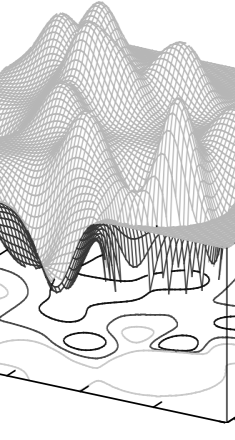
\includegraphics[height=7cm]{classPicture2-bw}
    }{\center

      \textbf{\fontsize{17}{20}\selectfont \course}

      ~

      %Lecture
      \topic\\

      \vspace{1cm}

      {\tiny~\emph{\keywords}~\\}

      \vspace{1cm}

      Marc Toussaint
      
      University of Stuttgart

      Summer 2019

      ~

    }
  }
}

\newcommand{\slide}[2]{
  \slidefont
  \incpage\begin{frame}
  \addcontentsline{toc}{section}{#1}
  \vfill
  {\headerfont #1} \vspace*{-2ex}
  \begin{itemize}\item[]~\\
    #2
  \end{itemize}
  \vfill
  \end{frame}
}

\newenvironment{slidecore}[1]{
  \slidefont\incpage
  \addcontentsline{toc}{section}{#1}
  \vfill
  {\headerfont #1} \vspace*{-2ex}
  \begin{itemize}\item[]~\\
}{
  \end{itemize}
  \vfill
}


\providecommand{\key}[1]{
  \addtocounter{mypage}{1}
% \immediate\write\keyfile{#1}
  \addtocontents{toc}{\hyperref[key:#1]{#1 (\arabic{mypage})}}
%  \phantomsection\label{key:#1}
%  \index{#1@{\hyperref[key:#1]{#1 (\arabic{mysec}:\arabic{mypage})}}|phantom}
  \addtocounter{mypage}{-1}
}

\providecommand{\course}{}

\providecommand{\subtopic}{}

\providecommand{\sublecture}[2]{
  \renewcommand{\subtopic}{#1}
  \slide{#1}{#2}
}

\providecommand{\story}[1]{
~

Motivation: {\tiny #1}\clearpage
}

\newenvironment{items}[1][9]{
\par\setlength{\unitlength}{1pt}\fontsize{#1}{#1}\linespread{1.2}\selectfont
\begin{list}{--}{\leftmargin4ex \rightmargin0ex \labelsep1ex \labelwidth2ex
\topsep0pt \parsep0ex \itemsep3pt}
}{
\end{list}
}

\providecommand{\slidesfoot}{
  \end{document}
}


  \slideshead
}

\providecommand{\exercises}{
  \newcommand{\exerciseshead}{
  \documentclass[10pt,fleqn]{article}
  \stdpackages

  \definecolor{bluecol}{rgb}{0,0,.5}
  \definecolor{greencol}{rgb}{0,.4,0}
  \definecolor{shadecolor}{gray}{0.9}
  \usepackage[
    %    pdftex%,
    %%    letterpaper,
    %    bookmarks,
    %    bookmarksnumbered,
    colorlinks,
    urlcolor=bluecol,
    citecolor=black,
    linkcolor=bluecol,
    %    pagecolor=bluecol,
    pdfborder={0 0 0},
    %pdfborderstyle={/S/U/W 1},
    %%    backref,     %link from bibliography back to sections
    %%    pagebackref, %link from bibliography back to pages
    %%    pdfstartview=FitH, %fitwidth instead of fit window
    pdfpagemode=UseNone, %UseOutlines, %bookmarks are displayed by acrobat
    pdftitle={\course},
    pdfauthor={Marc Toussaint},
    pdfkeywords={}
  ]{hyperref}
  \DeclareGraphicsExtensions{.pdf,.png,.jpg,.eps}

  \renewcommand{\r}{\varrho}
  \renewcommand{\l}{\lambda}
  \renewcommand{\L}{\Lambda}
  \renewcommand{\b}{\beta}
  \renewcommand{\d}{\delta}
  \renewcommand{\k}{\kappa}
  \renewcommand{\t}{\theta}
  \renewcommand{\O}{\Omega}
  \renewcommand{\o}{\omega}
  \renewcommand{\SS}{{\cal S}}
  \renewcommand{\=}{\!=\!}
  %\renewcommand{\boldsymbol}{}
  %\renewcommand{\Chapter}{\chapter}
  %\renewcommand{\Subsection}{\subsection}

  \renewcommand{\baselinestretch}{1.1}
  \geometry{a4paper,headsep=7mm,hdivide={15mm,*,15mm},vdivide={20mm,*,15mm}}

  \fancyhead[L]{\thetitle, \textit{Marc Toussaint}---\today}
  \fancyhead[R]{\thepage}
  \fancyhead[C]{}
  \fancyfoot{}
  \pagestyle{fancy}

  \parindent 0pt
  \parskip 0.5ex

  \newcommand{\codefont}{\helvetica{8}{1.2}{m}{n}}

  %auto-ignore
  \renewcommand{\a}{\alpha}
  \renewcommand{\b}{\beta}
  \renewcommand{\d}{\delta}
    \newcommand{\D}{\Delta}
    \newcommand{\e}{\epsilon}
    \newcommand{\g}{\gamma}
    \newcommand{\G}{\Gamma}
  \renewcommand{\l}{\lambda}
  \renewcommand{\L}{\Lambda}
    \newcommand{\m}{\mu}
    \newcommand{\n}{\nu}
    \newcommand{\N}{\nabla}
  \renewcommand{\k}{\kappa}
  \renewcommand{\o}{\omega}
  \renewcommand{\O}{\Omega}
    \newcommand{\p}{\phi}
    \newcommand{\ph}{\varphi}
  \renewcommand{\P}{\Phi}
  \renewcommand{\r}{\varrho}
    \newcommand{\s}{\sigma}
  \renewcommand{\S}{\Sigma}
  \renewcommand{\t}{\theta}
    \newcommand{\T}{\Theta}
  %\renewcommand{\v}{\vartheta}
    \newcommand{\x}{\xi}
    \newcommand{\X}{\Xi}
    \newcommand{\Y}{\Upsilon}
    \newcommand{\z}{\zeta}

  \renewcommand{\AA}{{\cal A}}
    \newcommand{\BB}{{\cal B}}
    \newcommand{\CC}{{\cal C}}
    \newcommand{\cc}{{\cal c}}
    \newcommand{\DD}{{\cal D}}
    \newcommand{\EE}{{\cal E}}
    \newcommand{\FF}{{\cal F}}
    \newcommand{\GG}{{\cal G}}
    \newcommand{\HH}{{\cal H}}
    \newcommand{\II}{{\cal I}}
    \newcommand{\KK}{{\cal K}}
    \newcommand{\LL}{{\cal L}}
    \newcommand{\MM}{{\cal M}}
    \newcommand{\NN}{{\cal N}}
    \newcommand{\oNN}{\overline\NN}
    \newcommand{\OO}{{\cal O}}
    \newcommand{\PP}{{\cal P}}
    \newcommand{\QQ}{{\cal Q}}
    \newcommand{\RR}{{\cal R}}
  \renewcommand{\SS}{{\cal S}}
    \newcommand{\TT}{{\cal T}}
    \newcommand{\uu}{{\cal u}}
    \newcommand{\UU}{{\cal U}}
    \newcommand{\VV}{{\cal V}}
    \newcommand{\XX}{{\cal X}}
    \newcommand{\xx}{\mathcal{x}}
    \newcommand{\YY}{{\cal Y}}
    \newcommand{\SOSO}{{\cal SO}}
    \newcommand{\GLGL}{{\cal GL}}

    \newcommand{\Ee}{{\rm E}}

  \newcommand{\NNN}{{\mathbb{N}}}
  \newcommand{\III}{{\mathbb{I}}}
  \newcommand{\ZZZ}{{\mathbb{Z}}}
  %\newcommand{\RRR}{{\mathrm{I\!R}}}
  \newcommand{\RRR}{{\mathbb{R}}}
  \newcommand{\SSS}{{\mathbb{S}}}
  \newcommand{\CCC}{{\mathbb{C}}}
  \newcommand{\DDD}{{\mathbb{D}}}
  \newcommand{\one}{{{\bf 1}}}
  \newcommand{\eee}{\text{e}}

  \newcommand{\NNNN}{{\overline{\cal N}}}

  \renewcommand{\[}{\Big[}
  \renewcommand{\]}{\Big]}
  \renewcommand{\(}{\Big(}
  \renewcommand{\)}{\Big)}
  \renewcommand{\|}{\,|\,}
  \renewcommand{\;}{\,;\,}
  \renewcommand{\=}{\!=\!}
    \newcommand{\<}{\left\langle}
  \renewcommand{\>}{\right\rangle}

  \newcommand{\na}[1][]{{\nabla_{\!\!#1}}}
  \newcommand{\he}[1][]{{\nabla_{\!\!#1}^2}}
  \newcommand{\Prob}{{\rm Prob}}
  \newcommand{\Dir}{{\rm Dir}}
  \newcommand{\Beta}{{\rm Beta}}
  \newcommand{\Bern}{{\rm Bern}}
  \newcommand{\Bin}{{\rm Bin}}
  \newcommand{\Mult}{{\rm Mult}}
  \newcommand{\Aut}{{\rm Aut}}
  \newcommand{\cor}{{\rm cor}}
  \newcommand{\corr}{{\rm corr}}
  \newcommand{\sd}{{\rm sd}}
  \newcommand{\tr}{{\rm tr}}
  \newcommand{\Tr}{{\rm Tr}}
  \newcommand{\rank}{{\rm rank}}
  \newcommand{\diag}{{\rm diag}}
  \newcommand{\dom}{{\rm dom}}
  \newcommand{\id}{{\rm id}}
  \newcommand{\Id}{{\rm\bf I}}
  \newcommand{\Gl}{{\rm Gl}}
  \renewcommand{\th}{\ensuremath{{}^\text{th}} }
  \newcommand{\lag}{\mathcal{L}}
  \newcommand{\inn}{\rfloor}
  \newcommand{\lie}{\pounds}
  \newcommand{\longto}{\longrightarrow}
  \newcommand{\speer}{\parbox{0.4ex}{\raisebox{0.8ex}{$\nearrow$}}}
  \renewcommand{\dag}{ {}^\dagger }
  \newcommand{\blbox}{\rule{1ex}{1ex}}
  \newcommand{\Ji}{J^\sharp}
  \newcommand{\h}{{}^\star}
  \newcommand{\w}{\wedge}
  \newcommand{\too}{\longrightarrow}
  \newcommand{\oot}{\longleftarrow}
  \newcommand{\To}{\Rightarrow}
  \newcommand{\oT}{\Leftarrow}
  \newcommand{\oTo}{\Leftrightarrow}
  \renewcommand{\iff}{~\Longleftrightarrow~}
  \newcommand{\Too}{\;\Longrightarrow\;}
  \newcommand{\oto}{\leftrightarrow}
  \newcommand{\ot}{\leftarrow}
  \newcommand{\ootoo}{\longleftrightarrow}
  \newcommand{\ow}{\stackrel{\circ}\wedge}
  \newcommand{\defeq}{\stackrel{\hspace{0.2ex}{}_\Delta}=}
%  \newcommand{\defeq}{{\overstack\Delta =}}
  \newcommand{\feed}{\nonumber \\}
  \newcommand{\comma}{~,\quad}
  \newcommand{\period}{~.\quad}
  \newcommand{\del}{\partial}
%  \newcommand{\quabla}{\Delta}
  \newcommand{\point}{$\bullet~~$}
  \newcommand{\doubletilde}{ ~ \raisebox{0.3ex}{$\widetilde {}$} \raisebox{0.6ex}{$\widetilde {}$} \!\! }
  \newcommand{\topcirc}{\parbox{0ex}{~\raisebox{2.5ex}{${}^\circ$}}}
  \newcommand{\topdot} {\parbox{0ex}{~\raisebox{2.5ex}{$\cdot$}}}
  \newcommand{\topddot} {\parbox{0ex}{~\raisebox{1.3ex}{$\ddot{~}$}}}
  \newcommand{\sym}{\topcirc}
  \newcommand{\tsum}{\textstyle\sum}
  \newcommand{\st}{\quad\text{s.t.}\quad}

  \newcommand{\half}{\ensuremath{\frac{1}{2}}}
  \newcommand{\third}{\ensuremath{\frac{1}{3}}}
  \newcommand{\fourth}{\ensuremath{\frac{1}{4}}}

  \newcommand{\ubar}{\underline}
  %\renewcommand{\vec}{\underline}
  \renewcommand{\vec}{\boldsymbol}
  %\renewcommand{\_}{\underset}
  %\renewcommand{\^}{\overset}
  %\renewcommand{\*}{{\rm\raisebox{-.6ex}{\text{*}}{}}}
  \renewcommand{\*}{\text{\footnotesize\raisebox{-.4ex}{*}{}}}

  \newcommand{\gto}{{\raisebox{.5ex}{${}_\rightarrow$}}}
  \newcommand{\gfrom}{{\raisebox{.5ex}{${}_\leftarrow$}}}
  \newcommand{\gnto}{{\raisebox{.5ex}{${}_\nrightarrow$}}}
  \newcommand{\gnfrom}{{\raisebox{.5ex}{${}_\nleftarrow$}}}

  %\newcommand{\RND}{{\SS}}
  %\newcommand{\IF}{\text{if }}
  %\newcommand{\AND}{\textsc{and }}
  %\newcommand{\OR}{\textsc{or }}
  %\newcommand{\XOR}{\textsc{xor }}
  %\newcommand{\NOT}{\textsc{not }}

  %\newcommand{\argmax}[1]{{\rm arg}\!\max_{#1}}
  %\newcommand{\argmin}[1]{{\rm arg}\!\min_{#1}}
  \DeclareMathOperator*{\argmax}{argmax}
  \DeclareMathOperator*{\argmin}{argmin}
  \DeclareMathOperator{\sign}{sign}
  \DeclareMathOperator{\acos}{acos}
  \DeclareMathOperator{\unifies}{unifies}
  \DeclareMathOperator{\Span}{span}
  \newcommand{\ortho}{\perp}
  %\newcommand{\argmax}[1]{\underset{~#1}{\text{argmax}}\;}
  %\newcommand{\argmin}[1]{\underset{~#1}{\text{argmin}}\;}
  \newcommand{\ee}[1]{\ensuremath{\cdot10^{#1}}}
  \newcommand{\sub}[1]{\ensuremath{_{\text{#1}}}}
  \newcommand{\up}[1]{\ensuremath{^{\text{#1}}}}
  \newcommand{\kld}[3][{}]{D_{#1}\big(#2\,\big|\!\big|\,#3\big)}
  %\newcommand{\kld}[2]{D\big(#1:#2\big)}
  \newcommand{\sprod}[2]{\big<#1\,,\,#2\big>}
  \newcommand{\End}{\text{End}}
  \newcommand{\txt}[1]{\quad\text{#1}\quad}
  \newcommand{\Over}[2]{\genfrac{}{}{0pt}{0}{#1}{#2}}
  %\newcommand{\mat}[1]{{\bf #1}}
  \newcommand{\arr}[2]{\hspace*{-.5ex}\begin{array}{#1}#2\end{array}\hspace*{-.5ex}}
  \newcommand{\mat}[3][.9]{
    \renewcommand{\arraystretch}{#1}{\scriptscriptstyle{\left(
      \hspace*{-1ex}\begin{array}{#2}#3\end{array}\hspace*{-1ex}
    \right)}}\renewcommand{\arraystretch}{1.2}
  }
  \newcommand{\Mat}[3][.9]{
    \renewcommand{\arraystretch}{#1}{\scriptscriptstyle{\left[
      \hspace*{-1ex}\begin{array}{#2}#3\end{array}\hspace*{-1ex}
    \right]}}\renewcommand{\arraystretch}{1.2}
  }
  \newcommand{\case}[2][ll]{\left\{\arr{#1}{#2}\right.}
  \newcommand{\seq}[1]{\textsf{\<#1\>}}
  \newcommand{\seqq}[1]{\textsf{#1}}
  \newcommand{\floor}[1]{\lfloor#1\rfloor}
  \newcommand{\Exp}[2][]{\text{E}_{#1}\{#2\}}
  \newcommand{\Var}[2][]{\text{Var}_{#1}\{#2\}}
  \newcommand{\cov}[2][]{\text{cov}_{#1}\{#2\}}

  %\newcommand{\Exp}[2]{\left\langle{#2}\right\rangle_{#1}}
  \newcommand{\ex}{\setminus}

  \providecommand{\href}[2]{{\color{blue}USE PDFLATEX!}}
  \providecommand{\url}[2]{\href{#1}{{\color{blue}#2}}}
%  \newcommand{\link}[1]{\href{{\protect #1}}{\texttt{\protect #1}}}
  \newcommand{\anchor}[2]{\begin{picture}(0,0)\put(#1){#2}\end{picture}}
  \newcommand{\pagebox}{\begin{picture}(0,0)\put(-3,-23){
    \textcolor[rgb]{.5,1,.5}{\framebox[\textwidth]{\rule[-\textheight]{0pt}{0pt}}}}
    \end{picture}}

  \newcommand{\hide}[1]{
    \begin{list}{}{\leftmargin0ex \rightmargin0ex \topsep0ex \parsep0ex}
       \helvetica{5}{1}{m}{n}
       \renewcommand{\section}{\par SECTION: }
       \renewcommand{\subsection}{\par SUBSECTION: }
       \item[$~~\blacktriangleright$]
       #1%$\blacktriangleleft~~$
       \message{^^JHIDE--Warning!^^J}
    \end{list}
  }
  %\newcommand{\hide}[1]{{\tt[hide:~}{\footnotesize\sf #1}{\tt]}\message{^^JHIDE--Warning!^^J}}
  \newcommand{\Hide}{\renewcommand{\hide}[1]{\message{^^JHIDE--Warning (hidden)!^^J}}}
  \newcommand{\HIDE}{\renewcommand{\hide}[1]{}}
  \newcommand{\fullhide}[1]{\message{^^JHIDE--Warning (hidden)!^^J}}
  \newcommand{\todo}[1]{{\tt[TODO: #1]}\message{^^JTODO--Warning: #1^^J}}
  \newcommand{\Todo}{\renewcommand{\todo}[1]{\message{^^JTODO--Warning (hidden)!^^J}}}
  %\renewcommand{\title}[1]{\renewcommand{\thetitle}{#1}}
  \newcommand{\myauthor}[1]{\author{#1}\newcommand{\theauthor}{#1}}%\@author}
  \newcommand{\mytitle}[1]{\title{#1}\newcommand{\thetitle}{#1}}%\@title}
  \newcommand{\header}{\begin{document}\mytitle\cleardefs}
  \newcommand{\contents}{{\tableofcontents}\renewcommand{\contents}{}}
  \newcommand{\footer}{\small\bibliography{marc,bibs}\end{document}}
  \newcommand{\widepaper}{\usepackage{geometry}\geometry{a4paper,hdivide={25mm,*,25mm},vdivide={25mm,*,25mm}}}
  \newcommand{\moviex}[2]{\movie[externalviewer]{#1}{#2}} %\pdflatex\usepackage{multimedia}
  \newcommand{\rbox}[1]{\fboxrule2mm\fcolorbox[rgb]{1,.85,.85}{1,.85,.85}{#1}}
  \newcommand{\mpage}[2]{{\begin{minipage}{#1\columnwidth}#2\end{minipage}}}
  \newcommand{\redbox}[2]{\fboxrule1mm\fcolorbox[rgb]{1,.7,.7}{1,.7,.7}{\begin{minipage}{#1\columnwidth}\center#2\end{minipage}}}
  \newcommand{\onecol}[2]{
    \begin{minipage}[c]{#1\columnwidth}#2\end{minipage}}
  \newcommand{\twocol}[5][0]{
    \begin{minipage}[c]{#2\columnwidth}#4\end{minipage}\hspace*{#1\columnwidth}%
    \begin{minipage}[c]{#3\columnwidth}#5\end{minipage}}
  \newcommand{\threecol}[7][0]{%
    \begin{minipage}[c]{#2\columnwidth}#5\end{minipage}\hspace*{#1\columnwidth}%
    \begin{minipage}[c]{#3\columnwidth}#6\end{minipage}\hspace*{#1\columnwidth}%
    \begin{minipage}[c]{#4\columnwidth}#7\end{minipage}}
  \newcommand{\threecoltext}[7][c]{
    \begin{minipage}[#1]{#2\textwidth}#5\end{minipage}%
    \begin{minipage}[#1]{#3\textwidth}#6\end{minipage}%
    \begin{minipage}[#1]{#4\textwidth}#7\end{minipage}}
  \newcommand{\threecoltop}[7][0]{%
   \begin{minipage}[t]{#2\columnwidth}#5\end{minipage}\hspace*{#1\columnwidth}%
   \begin{minipage}[t]{#3\columnwidth}#6\end{minipage}\hspace*{#1\columnwidth}%
   \begin{minipage}[t]{#4\columnwidth}#7\end{minipage}}
  \newcommand{\fourcol}[9][0]{%
   \begin{minipage}[c]{#2\columnwidth}#6\end{minipage}\hspace*{#1\columnwidth}%
   \begin{minipage}[c]{#3\columnwidth}#7\end{minipage}\hspace*{#1\columnwidth}%
   \begin{minipage}[c]{#4\columnwidth}#8\end{minipage}\hspace*{#1\columnwidth}%
   \begin{minipage}[c]{#5\columnwidth}#9\end{minipage}}
  \newcommand{\helvetica}[4]{\setlength{\unitlength}{1pt}\fontsize{#1}{#1}\linespread{#2}\usefont{OT1}{phv}{#3}{#4}}
  \newcommand{\helve}[1]{\helvetica{#1}{1.5}{m}{n}}
  \newcommand{\german}{\usepackage[german]{babel}\usepackage[utf8]{inputenc}}

\newcommand{\norm}[1]{|\!|#1|\!|}
\newcommand{\expr}[1]{[\hspace{-.2ex}[#1]\hspace{-.2ex}]}

\newcommand{\Jwi}{J^\sharp_W}
\newcommand{\THi}{T^\sharp_H}
\newcommand{\Jci}{J^\natural_C}
\newcommand{\hJi}{{\bar J}^\sharp}
\renewcommand{\|}{\,|\,}
\renewcommand{\=}{\!=\!}
\newcommand{\myminus}{{\hspace*{-.0pt}\text{\rm -}\hspace*{-.5pt}}}
\newcommand{\myplus}{{\hspace*{-.0pt}\text{\rm +}\hspace*{-.5pt}}}
\newcommand{\1}{{\myminus1}}
\newcommand{\2}{{\myminus2}}
\newcommand{\3}{{\myminus3}}
\newcommand{\mT}{{\text{\rm -}\hspace*{-1pt}\top}}
\newcommand{\po}{{\myplus1}}
\newcommand{\pt}{{\myplus2}}
%\renewcommand{\-}{\myminus}
%\newcommand{\+}{\myplus}
\renewcommand{\T}{{\!\top\!}}
\newcommand{\xT}{{\underline x}}
\newcommand{\uT}{{\underline u}}
\newcommand{\zT}{{\underline z}}
\newcommand{\Sum}{\textstyle\sum}
\newcommand{\Int}{\textstyle\int}
\newcommand{\Prod}{\textstyle\prod}


\newenvironment{centy}{
\vspace{15mm}
\large
\hspace*{5mm}
\begin{minipage}{8cm}\it\color{blue}
}{
\end{minipage}
}

\newcommand{\old}{{\text{old}}}
\newcommand{\new}{{\text{new}}}
\newcommand{\MAP}{{\text{MAP}}}
\newcommand{\ML}{{\text{ML}}}

\newcommand{\redArrow}{\quad\anchor{0,-1}{\includegraphics[scale=.5]{figs/redArrow}}}
\newcommand{\pub}[1]{{\color{green}\helvetica{8}{1.3}{m}{n}#1\\}}
\DeclareMathOperator{\opKL}{KL}
\newcommand{\KL}[2]{\opKL\big(#1\,\big|\!\big|\,#2\big)} %\left(#1 |\!| #2\right)}

\renewcommand{\show}[2][.8]{\centerline{\includegraphics[width=#1\columnwidth]{#2}}}
\newcommand{\showh}[2][.8]{\includegraphics[width=#1\columnwidth]{#2}}
\newcommand{\shows}[2][.8]{\centerline{\includegraphics[scale=#1]{#2}}}
\newcommand{\showhs}[2][.8]{\includegraphics[scale=#1]{#2}}
\newcommand{\mov}[2]{\movie[externalviewer]{{\color{blue}\small #1}}{movies/#2}}
\newcommand{\movex}[2]{\movie[externalviewer]{#1}{#2}} %\pdflatex\usepackage{multimedia}
%\newcommand{\movgb}[1]{\hfill\movie[externalviewer]{\small[movie]}{/home/mtoussai/movies/10-goalDirectedBehavior/#1}}
\newcommand{\movh}[3][loop]{
\movie[#1]{\showh[#2]{movies/#3.png}}{movies/#3.avi}%
\movie[externalviewer]{$\circ$}{movies/#3.avi}
}
\newcommand{\movc}[3][loop]{\centerline{\movh[#1]{#2}{#3}}}
\newcommand{\cen}[1]{\centerline{#1}}

\newcommand{\citing}[1]{
{\color{citcol}\tiny#1\par}
}

\newcommand{\cit}[3]{
\par\smallskip
{\color{greencol}\tiny #1: \emph{#2}. #3 \par}
}

\newcommand{\citurl}[4]{
\par\smallskip
{\color{greencol}\tiny #1: \protect{\href{#4}{\color{blue}{#2.}}} #3 \par}
}

\newcommand{\cito}[3]{
\par\smallskip
{\color{bluecol}\tiny #1: \emph{#2}. #3 \par}
}

\newcommand{\redoMacrosInProof}{
  \renewcommand{\d}{\delta}
%  \renewcommand{\|}{\,|\,}
  \renewcommand{\=}{\!=\!}
}

%% \makeatletter
%% \newenvironment{code}{%
%%   \begin{lrbox}{\@tempboxa}\begin{minipage}{1\columnwidth}\codefont
%% }{
%%   \end{minipage}\end{lrbox}%
%%   \colorbox[rgb]{.95,.95,.95}{\usebox{\@tempboxa}}
%% }\makeatother

\newenvironment{code}{%
\codefont
\begin{shaded}
}{
\end{shaded}
}

%\newcommand{\refeq}[1]{(\ref{#1})}

\usepackage{algorithm}
\usepackage{algpseudocode}
\algrenewcommand{\algorithmicrequire}{\textbf{Input:~~}}
\algrenewcommand{\algorithmicensure}{\textbf{Output:}}
\algrenewcommand{\algorithmiccomment}[1]{\qquad\hfill~\hspace*{-5ex}\textit{// #1}}
\algrenewcommand{\alglinenumber}[1]{\helvetica{6}{1.3}{m}{n}#1:}

\newenvironment{algo}[1][8]{
\quad\begin{minipage}{.8\columnwidth}\helvetica{#1}{1.3}{m}{n}
\medskip\hrule\medskip
\begin{algorithmic}[1]
}{
\end{algorithmic}
\medskip\hrule\medskip
\end{minipage}
}

\usepackage{etoolbox}

%%%%%%%%%%%%%%%%%%%%%%%%%%%%%%%%%%%%%%%%%%%%%%%%%%%%%%%%%%%%%%%%%%%%%%%%%%%%%%%%

\usepackage{multirow}
\usepackage{colortbl}
%\setlength{\jot}{0pt}
%\setlength{\mathindent}{1ex}
\usepackage{empheq}

%%%%%%%%%%%%%%%%%%%%%%%%%%%%%%%%%%%%%%%%%%%%%%%%%%%%%%%%%%%%%%%%%%%%%%%%%%%%%%%

\newcommand{\mypause}{\pause}
%\newcommand{\dom}{{\text{dom}}}
\newcommand{\defi}[1]{\textbf{#1}}
\newcommand{\red}[1]{\emph{\color{red}#1}}
%\newcommand{\ul}{\underline}
\newcommand{\pos}{{\textsf{pos}}}
\newcommand{\eff}{{\textsf{eff}}}
\newcommand{\rot}{{\textsf{rot}}}
\newcommand{\veC}{{\textsf{vec}}}
\newcommand{\quat}{{\textsf{quat}}}
\newcommand{\col}{{\textsf{col}}}
\newcommand{\de}[2]{\frac{\partial #1}{\partial #2}}
\newcommand{\target}{{\text{target}}}
\newcommand{\near}{{\text{near}}}
\newcommand{\qfree}{Q_{\text{free}}}
\renewcommand{\vec}{\boldsymbol}
\newcommand{\lft}{\text{left}}
\newcommand{\rgh}{\text{right}}
\DeclareMathOperator{\real}{real}
\newcommand{\prev}{{\text{prev}}}
\newcommand{\TR}[2]{T_{{#1}\shortrightarrow{#2}}}
\newcommand{\RO}[2]{R_{{#1}\shortrightarrow{#2}}}
\newcommand{\liter}{\helvetica{8}{1.1}{m}{n}\parskip 1ex}
\newcommand{\Fc}{\color{green}F}
\newcommand{\muc}{\color{blue}\mu}
\newcommand{\Astar}{A$^*$}

%for optimization course:
\newcommand{\adec}{\r_\a^-}
\newcommand{\ainc}{\r_\a^+}
\newcommand{\ldec}{\r_\l^-}
\newcommand{\linc}{\r_\l^+}
\newcommand{\minc}{\r_\m^+}
\newcommand{\mdec}{\r_\m^-}
\newcommand{\lsstop}{\r_{\text{ls}}}


\definecolor{boxcol}{rgb}{.85,.9,.92}
\newcommand{\eqbox}[1]{\centerline{\fboxrule0mm\fcolorbox{boxcol}{boxcol}{#1}}}
\newcommand{\movgb}[1]{\hfill\movie[externalviewer]{\small[movie]}{/home/mtoussai/movies/10-goalDirectedBehavior/#1}}
\newcommand{\demo}[1]{{{\color{blue}[\small #1]}}}

\graphicspath{{../pics-robotics/}{../pics-ML/}{../pics-all/}{../pics-all2/}{../pics-Optim/}}
\DeclareGraphicsExtensions{.pdf,.png,.jpg}

%\usepackage{pdfpages}
%\setbeamercolor{background canvas}{bg=}

\newcommand{\SUM}{\texttt{sum}}
\usepackage{float}

%% prevent pagebreaks before environment
\makeatletter
\newcommand{\NewParNoBreak}[1][\parskip]{\par\vspace*{-\parskip}\vspace*{#1}\nobreak\@afterheading}
\makeatother

%\newcommand{\idx}[2]{\label{IKgn}}

%%%%%%%%%%%%%%%%%%%%%%%%%%%%%%%%%%%%%%%%%%%%%%%%%%%%%%%%%%%%%%%%%%%%%%%%%%%%%%%%



%% \newwrite\tempfile
%% \immediate\openout\tempfile=z.keys.tex

%% \renewcommand{\key}[1]{
%% %%   \addtocounter{mypage}{1}
%% \makeatletter
%% \immediate\write\tempfile{\symbol{`\\}}
%% \makeatother
%%   \immediate\write\tempfile{hyperref[key:#1]{#1(\arabic{mypage})}}
%% %%  % \phantomsection\label{key:#1}
%% %%   %\index{#1@{\hyperref[key:#1]{#1 (\arabic{mysec}:\arabic{mypage})}}|phantom}
%% %%   \addtocounter{mypage}{-1}
%% }


  \DefineShortVerb{\@}

  \newcounter{solutions}
  \setcounter{solutions}{1}
  \newenvironment{solution}{
    \small
    \begin{shaded}
  }{
    \end{shaded}
  }
  
  \renewcommand{\hat}{\widehat}
  \newcommand{\bbg}{{\bar{\bar g}}}
  \graphicspath{{pics/}{../shared/pics/}}

  \renewcommand{\labelenumi}{{\alph{enumi})}}

  %%%%%%%%%%%%%%%%%%%%%%%%%%%%%%%%%%%%%%%%%%%%%%%%%%%%%%%%%%%%%%%%%%%%%%%%%%%%%%%%


  \mytitle{\course\\Exercise \exnum}
  \myauthor{Marc Toussaint\\ TAs: Janik Hager, Philipp Kratzer\\\small\addressUSTT}
  
  
  \begin{document}
  \onecolumn
  \maketitle
}

\newcommand{\exsection}[1]{\section{#1}}

\newcommand{\exerfoot}{
  \end{document}
}

\newenvironment{items}[1][9]{
  \par\setlength{\unitlength}{1pt}\fontsize{#1}{#1}\linespread{1.2}\selectfont
  \begin{list}{--}{\leftmargin4ex \rightmargin0ex \labelsep1ex \labelwidth2ex
      \topsep0pt \parsep0ex \itemsep3pt}
}{
  \end{list}
}

  \exerciseshead
}

\providecommand{\script}{
  \newcommand{\scripthead}{
  \documentclass[9pt,twoside]{article}
  \stdpackages

  \usepackage{palatino}
  \usepackage[envcountsect]{beamerarticle}
  \usepackage{makeidx}
  \makeindex

  \definecolor{bluecol}{rgb}{0,0,.5}
  \definecolor{greencol}{rgb}{0,.4,0}
  \definecolor{shadecolor}{gray}{0.9}
  \usepackage[
    %    pdftex%,
    %%    letterpaper,
    %bookmarks,
    bookmarksnumbered,
    colorlinks,
    urlcolor=bluecol,
    citecolor=black,
    linkcolor=bluecol,
    %    pagecolor=bluecol,
    pdfborder={0 0 0},
    %pdfborderstyle={/S/U/W 1},
    %%    backref,     %link from bibliography back to sections
    %%    pagebackref, %link from bibliography back to pages
    %%    pdfstartview=FitH, %fitwidth instead of fit window
    pdfpagemode=UseOutlines, %bookmarks are displayed by acrobat
    pdftitle={\course},
    pdfauthor={Marc Toussaint},
    pdfkeywords={}
  ]{hyperref}
  \DeclareGraphicsExtensions{.pdf,.png,.jpg,.eps}

  \usepackage{multimedia}
  %\setbeamercolor{background canvas}{bg=}

  \renewcommand{\r}{\varrho}
  \renewcommand{\l}{\lambda}
  \renewcommand{\L}{\Lambda}
  \renewcommand{\b}{\beta}
  \renewcommand{\d}{\delta}
  \renewcommand{\k}{\kappa}
  \renewcommand{\t}{\theta}
  \renewcommand{\O}{\Omega}
  \renewcommand{\o}{\omega}
  \renewcommand{\SS}{{\cal S}}
  \renewcommand{\=}{\!=\!}
  %\renewcommand{\boldsymbol}{}
  %\renewcommand{\Chapter}{\chapter}
  %\renewcommand{\Subsection}{\subsection}

  \renewcommand{\baselinestretch}{1.0}
  \geometry{a5paper,headsep=6mm,hdivide={10mm,*,10mm},vdivide={13mm,*,7mm}}

  \fancyhead[OL,ER]{\course, \textit{Marc Toussaint}}
  \fancyhead[OR,EL]{\thepage}
  \fancyhead[C]{}
  \fancyfoot{}
  \pagestyle{fancy}

%  \setcounter{tocdepth}{3}
  \setcounter{tocdepth}{2}

   \columnsep 6ex
  %  \renewcommand{\familydefault}{\sfdefault}
  \newcommand{\headerfont}{\large}%helvetica{12}{1}{b}{n}}
  \newcommand{\slidefont} {}%\helvetica{9}{1.3}{m}{n}}
  \newcommand{\storyfont} {}
  %  \renewcommand{\small}   {\helvetica{8}{1.2}{m}{n}}
  \renewcommand{\tiny}    {\footnotesize}%helvetica{7}{1.1}{m}{n}}
  \newcommand{\codefont}{\fontsize{6}{6}\selectfont}%helvetica{8}{1.2}{m}{n}}

  %auto-ignore
  \renewcommand{\a}{\alpha}
  \renewcommand{\b}{\beta}
  \renewcommand{\d}{\delta}
    \newcommand{\D}{\Delta}
    \newcommand{\e}{\epsilon}
    \newcommand{\g}{\gamma}
    \newcommand{\G}{\Gamma}
  \renewcommand{\l}{\lambda}
  \renewcommand{\L}{\Lambda}
    \newcommand{\m}{\mu}
    \newcommand{\n}{\nu}
    \newcommand{\N}{\nabla}
  \renewcommand{\k}{\kappa}
  \renewcommand{\o}{\omega}
  \renewcommand{\O}{\Omega}
    \newcommand{\p}{\phi}
    \newcommand{\ph}{\varphi}
  \renewcommand{\P}{\Phi}
  \renewcommand{\r}{\varrho}
    \newcommand{\s}{\sigma}
  \renewcommand{\S}{\Sigma}
  \renewcommand{\t}{\theta}
    \newcommand{\T}{\Theta}
  %\renewcommand{\v}{\vartheta}
    \newcommand{\x}{\xi}
    \newcommand{\X}{\Xi}
    \newcommand{\Y}{\Upsilon}
    \newcommand{\z}{\zeta}

  \renewcommand{\AA}{{\cal A}}
    \newcommand{\BB}{{\cal B}}
    \newcommand{\CC}{{\cal C}}
    \newcommand{\cc}{{\cal c}}
    \newcommand{\DD}{{\cal D}}
    \newcommand{\EE}{{\cal E}}
    \newcommand{\FF}{{\cal F}}
    \newcommand{\GG}{{\cal G}}
    \newcommand{\HH}{{\cal H}}
    \newcommand{\II}{{\cal I}}
    \newcommand{\KK}{{\cal K}}
    \newcommand{\LL}{{\cal L}}
    \newcommand{\MM}{{\cal M}}
    \newcommand{\NN}{{\cal N}}
    \newcommand{\oNN}{\overline\NN}
    \newcommand{\OO}{{\cal O}}
    \newcommand{\PP}{{\cal P}}
    \newcommand{\QQ}{{\cal Q}}
    \newcommand{\RR}{{\cal R}}
  \renewcommand{\SS}{{\cal S}}
    \newcommand{\TT}{{\cal T}}
    \newcommand{\uu}{{\cal u}}
    \newcommand{\UU}{{\cal U}}
    \newcommand{\VV}{{\cal V}}
    \newcommand{\XX}{{\cal X}}
    \newcommand{\xx}{\mathcal{x}}
    \newcommand{\YY}{{\cal Y}}
    \newcommand{\SOSO}{{\cal SO}}
    \newcommand{\GLGL}{{\cal GL}}

    \newcommand{\Ee}{{\rm E}}

  \newcommand{\NNN}{{\mathbb{N}}}
  \newcommand{\III}{{\mathbb{I}}}
  \newcommand{\ZZZ}{{\mathbb{Z}}}
  %\newcommand{\RRR}{{\mathrm{I\!R}}}
  \newcommand{\RRR}{{\mathbb{R}}}
  \newcommand{\SSS}{{\mathbb{S}}}
  \newcommand{\CCC}{{\mathbb{C}}}
  \newcommand{\DDD}{{\mathbb{D}}}
  \newcommand{\one}{{{\bf 1}}}
  \newcommand{\eee}{\text{e}}

  \newcommand{\NNNN}{{\overline{\cal N}}}

  \renewcommand{\[}{\Big[}
  \renewcommand{\]}{\Big]}
  \renewcommand{\(}{\Big(}
  \renewcommand{\)}{\Big)}
  \renewcommand{\|}{\,|\,}
  \renewcommand{\;}{\,;\,}
  \renewcommand{\=}{\!=\!}
    \newcommand{\<}{\left\langle}
  \renewcommand{\>}{\right\rangle}

  \newcommand{\na}[1][]{{\nabla_{\!\!#1}}}
  \newcommand{\he}[1][]{{\nabla_{\!\!#1}^2}}
  \newcommand{\Prob}{{\rm Prob}}
  \newcommand{\Dir}{{\rm Dir}}
  \newcommand{\Beta}{{\rm Beta}}
  \newcommand{\Bern}{{\rm Bern}}
  \newcommand{\Bin}{{\rm Bin}}
  \newcommand{\Mult}{{\rm Mult}}
  \newcommand{\Aut}{{\rm Aut}}
  \newcommand{\cor}{{\rm cor}}
  \newcommand{\corr}{{\rm corr}}
  \newcommand{\sd}{{\rm sd}}
  \newcommand{\tr}{{\rm tr}}
  \newcommand{\Tr}{{\rm Tr}}
  \newcommand{\rank}{{\rm rank}}
  \newcommand{\diag}{{\rm diag}}
  \newcommand{\dom}{{\rm dom}}
  \newcommand{\id}{{\rm id}}
  \newcommand{\Id}{{\rm\bf I}}
  \newcommand{\Gl}{{\rm Gl}}
  \renewcommand{\th}{\ensuremath{{}^\text{th}} }
  \newcommand{\lag}{\mathcal{L}}
  \newcommand{\inn}{\rfloor}
  \newcommand{\lie}{\pounds}
  \newcommand{\longto}{\longrightarrow}
  \newcommand{\speer}{\parbox{0.4ex}{\raisebox{0.8ex}{$\nearrow$}}}
  \renewcommand{\dag}{ {}^\dagger }
  \newcommand{\blbox}{\rule{1ex}{1ex}}
  \newcommand{\Ji}{J^\sharp}
  \newcommand{\h}{{}^\star}
  \newcommand{\w}{\wedge}
  \newcommand{\too}{\longrightarrow}
  \newcommand{\oot}{\longleftarrow}
  \newcommand{\To}{\Rightarrow}
  \newcommand{\oT}{\Leftarrow}
  \newcommand{\oTo}{\Leftrightarrow}
  \renewcommand{\iff}{~\Longleftrightarrow~}
  \newcommand{\Too}{\;\Longrightarrow\;}
  \newcommand{\oto}{\leftrightarrow}
  \newcommand{\ot}{\leftarrow}
  \newcommand{\ootoo}{\longleftrightarrow}
  \newcommand{\ow}{\stackrel{\circ}\wedge}
  \newcommand{\defeq}{\stackrel{\hspace{0.2ex}{}_\Delta}=}
%  \newcommand{\defeq}{{\overstack\Delta =}}
  \newcommand{\feed}{\nonumber \\}
  \newcommand{\comma}{~,\quad}
  \newcommand{\period}{~.\quad}
  \newcommand{\del}{\partial}
%  \newcommand{\quabla}{\Delta}
  \newcommand{\point}{$\bullet~~$}
  \newcommand{\doubletilde}{ ~ \raisebox{0.3ex}{$\widetilde {}$} \raisebox{0.6ex}{$\widetilde {}$} \!\! }
  \newcommand{\topcirc}{\parbox{0ex}{~\raisebox{2.5ex}{${}^\circ$}}}
  \newcommand{\topdot} {\parbox{0ex}{~\raisebox{2.5ex}{$\cdot$}}}
  \newcommand{\topddot} {\parbox{0ex}{~\raisebox{1.3ex}{$\ddot{~}$}}}
  \newcommand{\sym}{\topcirc}
  \newcommand{\tsum}{\textstyle\sum}
  \newcommand{\st}{\quad\text{s.t.}\quad}

  \newcommand{\half}{\ensuremath{\frac{1}{2}}}
  \newcommand{\third}{\ensuremath{\frac{1}{3}}}
  \newcommand{\fourth}{\ensuremath{\frac{1}{4}}}

  \newcommand{\ubar}{\underline}
  %\renewcommand{\vec}{\underline}
  \renewcommand{\vec}{\boldsymbol}
  %\renewcommand{\_}{\underset}
  %\renewcommand{\^}{\overset}
  %\renewcommand{\*}{{\rm\raisebox{-.6ex}{\text{*}}{}}}
  \renewcommand{\*}{\text{\footnotesize\raisebox{-.4ex}{*}{}}}

  \newcommand{\gto}{{\raisebox{.5ex}{${}_\rightarrow$}}}
  \newcommand{\gfrom}{{\raisebox{.5ex}{${}_\leftarrow$}}}
  \newcommand{\gnto}{{\raisebox{.5ex}{${}_\nrightarrow$}}}
  \newcommand{\gnfrom}{{\raisebox{.5ex}{${}_\nleftarrow$}}}

  %\newcommand{\RND}{{\SS}}
  %\newcommand{\IF}{\text{if }}
  %\newcommand{\AND}{\textsc{and }}
  %\newcommand{\OR}{\textsc{or }}
  %\newcommand{\XOR}{\textsc{xor }}
  %\newcommand{\NOT}{\textsc{not }}

  %\newcommand{\argmax}[1]{{\rm arg}\!\max_{#1}}
  %\newcommand{\argmin}[1]{{\rm arg}\!\min_{#1}}
  \DeclareMathOperator*{\argmax}{argmax}
  \DeclareMathOperator*{\argmin}{argmin}
  \DeclareMathOperator{\sign}{sign}
  \DeclareMathOperator{\acos}{acos}
  \DeclareMathOperator{\unifies}{unifies}
  \DeclareMathOperator{\Span}{span}
  \newcommand{\ortho}{\perp}
  %\newcommand{\argmax}[1]{\underset{~#1}{\text{argmax}}\;}
  %\newcommand{\argmin}[1]{\underset{~#1}{\text{argmin}}\;}
  \newcommand{\ee}[1]{\ensuremath{\cdot10^{#1}}}
  \newcommand{\sub}[1]{\ensuremath{_{\text{#1}}}}
  \newcommand{\up}[1]{\ensuremath{^{\text{#1}}}}
  \newcommand{\kld}[3][{}]{D_{#1}\big(#2\,\big|\!\big|\,#3\big)}
  %\newcommand{\kld}[2]{D\big(#1:#2\big)}
  \newcommand{\sprod}[2]{\big<#1\,,\,#2\big>}
  \newcommand{\End}{\text{End}}
  \newcommand{\txt}[1]{\quad\text{#1}\quad}
  \newcommand{\Over}[2]{\genfrac{}{}{0pt}{0}{#1}{#2}}
  %\newcommand{\mat}[1]{{\bf #1}}
  \newcommand{\arr}[2]{\hspace*{-.5ex}\begin{array}{#1}#2\end{array}\hspace*{-.5ex}}
  \newcommand{\mat}[3][.9]{
    \renewcommand{\arraystretch}{#1}{\scriptscriptstyle{\left(
      \hspace*{-1ex}\begin{array}{#2}#3\end{array}\hspace*{-1ex}
    \right)}}\renewcommand{\arraystretch}{1.2}
  }
  \newcommand{\Mat}[3][.9]{
    \renewcommand{\arraystretch}{#1}{\scriptscriptstyle{\left[
      \hspace*{-1ex}\begin{array}{#2}#3\end{array}\hspace*{-1ex}
    \right]}}\renewcommand{\arraystretch}{1.2}
  }
  \newcommand{\case}[2][ll]{\left\{\arr{#1}{#2}\right.}
  \newcommand{\seq}[1]{\textsf{\<#1\>}}
  \newcommand{\seqq}[1]{\textsf{#1}}
  \newcommand{\floor}[1]{\lfloor#1\rfloor}
  \newcommand{\Exp}[2][]{\text{E}_{#1}\{#2\}}
  \newcommand{\Var}[2][]{\text{Var}_{#1}\{#2\}}
  \newcommand{\cov}[2][]{\text{cov}_{#1}\{#2\}}

  %\newcommand{\Exp}[2]{\left\langle{#2}\right\rangle_{#1}}
  \newcommand{\ex}{\setminus}

  \providecommand{\href}[2]{{\color{blue}USE PDFLATEX!}}
  \providecommand{\url}[2]{\href{#1}{{\color{blue}#2}}}
%  \newcommand{\link}[1]{\href{{\protect #1}}{\texttt{\protect #1}}}
  \newcommand{\anchor}[2]{\begin{picture}(0,0)\put(#1){#2}\end{picture}}
  \newcommand{\pagebox}{\begin{picture}(0,0)\put(-3,-23){
    \textcolor[rgb]{.5,1,.5}{\framebox[\textwidth]{\rule[-\textheight]{0pt}{0pt}}}}
    \end{picture}}

  \newcommand{\hide}[1]{
    \begin{list}{}{\leftmargin0ex \rightmargin0ex \topsep0ex \parsep0ex}
       \helvetica{5}{1}{m}{n}
       \renewcommand{\section}{\par SECTION: }
       \renewcommand{\subsection}{\par SUBSECTION: }
       \item[$~~\blacktriangleright$]
       #1%$\blacktriangleleft~~$
       \message{^^JHIDE--Warning!^^J}
    \end{list}
  }
  %\newcommand{\hide}[1]{{\tt[hide:~}{\footnotesize\sf #1}{\tt]}\message{^^JHIDE--Warning!^^J}}
  \newcommand{\Hide}{\renewcommand{\hide}[1]{\message{^^JHIDE--Warning (hidden)!^^J}}}
  \newcommand{\HIDE}{\renewcommand{\hide}[1]{}}
  \newcommand{\fullhide}[1]{\message{^^JHIDE--Warning (hidden)!^^J}}
  \newcommand{\todo}[1]{{\tt[TODO: #1]}\message{^^JTODO--Warning: #1^^J}}
  \newcommand{\Todo}{\renewcommand{\todo}[1]{\message{^^JTODO--Warning (hidden)!^^J}}}
  %\renewcommand{\title}[1]{\renewcommand{\thetitle}{#1}}
  \newcommand{\myauthor}[1]{\author{#1}\newcommand{\theauthor}{#1}}%\@author}
  \newcommand{\mytitle}[1]{\title{#1}\newcommand{\thetitle}{#1}}%\@title}
  \newcommand{\header}{\begin{document}\mytitle\cleardefs}
  \newcommand{\contents}{{\tableofcontents}\renewcommand{\contents}{}}
  \newcommand{\footer}{\small\bibliography{marc,bibs}\end{document}}
  \newcommand{\widepaper}{\usepackage{geometry}\geometry{a4paper,hdivide={25mm,*,25mm},vdivide={25mm,*,25mm}}}
  \newcommand{\moviex}[2]{\movie[externalviewer]{#1}{#2}} %\pdflatex\usepackage{multimedia}
  \newcommand{\rbox}[1]{\fboxrule2mm\fcolorbox[rgb]{1,.85,.85}{1,.85,.85}{#1}}
  \newcommand{\mpage}[2]{{\begin{minipage}{#1\columnwidth}#2\end{minipage}}}
  \newcommand{\redbox}[2]{\fboxrule1mm\fcolorbox[rgb]{1,.7,.7}{1,.7,.7}{\begin{minipage}{#1\columnwidth}\center#2\end{minipage}}}
  \newcommand{\onecol}[2]{
    \begin{minipage}[c]{#1\columnwidth}#2\end{minipage}}
  \newcommand{\twocol}[5][0]{
    \begin{minipage}[c]{#2\columnwidth}#4\end{minipage}\hspace*{#1\columnwidth}%
    \begin{minipage}[c]{#3\columnwidth}#5\end{minipage}}
  \newcommand{\threecol}[7][0]{%
    \begin{minipage}[c]{#2\columnwidth}#5\end{minipage}\hspace*{#1\columnwidth}%
    \begin{minipage}[c]{#3\columnwidth}#6\end{minipage}\hspace*{#1\columnwidth}%
    \begin{minipage}[c]{#4\columnwidth}#7\end{minipage}}
  \newcommand{\threecoltext}[7][c]{
    \begin{minipage}[#1]{#2\textwidth}#5\end{minipage}%
    \begin{minipage}[#1]{#3\textwidth}#6\end{minipage}%
    \begin{minipage}[#1]{#4\textwidth}#7\end{minipage}}
  \newcommand{\threecoltop}[7][0]{%
   \begin{minipage}[t]{#2\columnwidth}#5\end{minipage}\hspace*{#1\columnwidth}%
   \begin{minipage}[t]{#3\columnwidth}#6\end{minipage}\hspace*{#1\columnwidth}%
   \begin{minipage}[t]{#4\columnwidth}#7\end{minipage}}
  \newcommand{\fourcol}[9][0]{%
   \begin{minipage}[c]{#2\columnwidth}#6\end{minipage}\hspace*{#1\columnwidth}%
   \begin{minipage}[c]{#3\columnwidth}#7\end{minipage}\hspace*{#1\columnwidth}%
   \begin{minipage}[c]{#4\columnwidth}#8\end{minipage}\hspace*{#1\columnwidth}%
   \begin{minipage}[c]{#5\columnwidth}#9\end{minipage}}
  \newcommand{\helvetica}[4]{\setlength{\unitlength}{1pt}\fontsize{#1}{#1}\linespread{#2}\usefont{OT1}{phv}{#3}{#4}}
  \newcommand{\helve}[1]{\helvetica{#1}{1.5}{m}{n}}
  \newcommand{\german}{\usepackage[german]{babel}\usepackage[utf8]{inputenc}}

\newcommand{\norm}[1]{|\!|#1|\!|}
\newcommand{\expr}[1]{[\hspace{-.2ex}[#1]\hspace{-.2ex}]}

\newcommand{\Jwi}{J^\sharp_W}
\newcommand{\THi}{T^\sharp_H}
\newcommand{\Jci}{J^\natural_C}
\newcommand{\hJi}{{\bar J}^\sharp}
\renewcommand{\|}{\,|\,}
\renewcommand{\=}{\!=\!}
\newcommand{\myminus}{{\hspace*{-.0pt}\text{\rm -}\hspace*{-.5pt}}}
\newcommand{\myplus}{{\hspace*{-.0pt}\text{\rm +}\hspace*{-.5pt}}}
\newcommand{\1}{{\myminus1}}
\newcommand{\2}{{\myminus2}}
\newcommand{\3}{{\myminus3}}
\newcommand{\mT}{{\text{\rm -}\hspace*{-1pt}\top}}
\newcommand{\po}{{\myplus1}}
\newcommand{\pt}{{\myplus2}}
%\renewcommand{\-}{\myminus}
%\newcommand{\+}{\myplus}
\renewcommand{\T}{{\!\top\!}}
\newcommand{\xT}{{\underline x}}
\newcommand{\uT}{{\underline u}}
\newcommand{\zT}{{\underline z}}
\newcommand{\Sum}{\textstyle\sum}
\newcommand{\Int}{\textstyle\int}
\newcommand{\Prod}{\textstyle\prod}


\newenvironment{centy}{
\vspace{15mm}
\large
\hspace*{5mm}
\begin{minipage}{8cm}\it\color{blue}
}{
\end{minipage}
}

\newcommand{\old}{{\text{old}}}
\newcommand{\new}{{\text{new}}}
\newcommand{\MAP}{{\text{MAP}}}
\newcommand{\ML}{{\text{ML}}}

\newcommand{\redArrow}{\quad\anchor{0,-1}{\includegraphics[scale=.5]{figs/redArrow}}}
\newcommand{\pub}[1]{{\color{green}\helvetica{8}{1.3}{m}{n}#1\\}}
\DeclareMathOperator{\opKL}{KL}
\newcommand{\KL}[2]{\opKL\big(#1\,\big|\!\big|\,#2\big)} %\left(#1 |\!| #2\right)}

\renewcommand{\show}[2][.8]{\centerline{\includegraphics[width=#1\columnwidth]{#2}}}
\newcommand{\showh}[2][.8]{\includegraphics[width=#1\columnwidth]{#2}}
\newcommand{\shows}[2][.8]{\centerline{\includegraphics[scale=#1]{#2}}}
\newcommand{\showhs}[2][.8]{\includegraphics[scale=#1]{#2}}
\newcommand{\mov}[2]{\movie[externalviewer]{{\color{blue}\small #1}}{movies/#2}}
\newcommand{\movex}[2]{\movie[externalviewer]{#1}{#2}} %\pdflatex\usepackage{multimedia}
%\newcommand{\movgb}[1]{\hfill\movie[externalviewer]{\small[movie]}{/home/mtoussai/movies/10-goalDirectedBehavior/#1}}
\newcommand{\movh}[3][loop]{
\movie[#1]{\showh[#2]{movies/#3.png}}{movies/#3.avi}%
\movie[externalviewer]{$\circ$}{movies/#3.avi}
}
\newcommand{\movc}[3][loop]{\centerline{\movh[#1]{#2}{#3}}}
\newcommand{\cen}[1]{\centerline{#1}}

\newcommand{\citing}[1]{
{\color{citcol}\tiny#1\par}
}

\newcommand{\cit}[3]{
\par\smallskip
{\color{greencol}\tiny #1: \emph{#2}. #3 \par}
}

\newcommand{\citurl}[4]{
\par\smallskip
{\color{greencol}\tiny #1: \protect{\href{#4}{\color{blue}{#2.}}} #3 \par}
}

\newcommand{\cito}[3]{
\par\smallskip
{\color{bluecol}\tiny #1: \emph{#2}. #3 \par}
}

\newcommand{\redoMacrosInProof}{
  \renewcommand{\d}{\delta}
%  \renewcommand{\|}{\,|\,}
  \renewcommand{\=}{\!=\!}
}

%% \makeatletter
%% \newenvironment{code}{%
%%   \begin{lrbox}{\@tempboxa}\begin{minipage}{1\columnwidth}\codefont
%% }{
%%   \end{minipage}\end{lrbox}%
%%   \colorbox[rgb]{.95,.95,.95}{\usebox{\@tempboxa}}
%% }\makeatother

\newenvironment{code}{%
\codefont
\begin{shaded}
}{
\end{shaded}
}

%\newcommand{\refeq}[1]{(\ref{#1})}

\usepackage{algorithm}
\usepackage{algpseudocode}
\algrenewcommand{\algorithmicrequire}{\textbf{Input:~~}}
\algrenewcommand{\algorithmicensure}{\textbf{Output:}}
\algrenewcommand{\algorithmiccomment}[1]{\qquad\hfill~\hspace*{-5ex}\textit{// #1}}
\algrenewcommand{\alglinenumber}[1]{\helvetica{6}{1.3}{m}{n}#1:}

\newenvironment{algo}[1][8]{
\quad\begin{minipage}{.8\columnwidth}\helvetica{#1}{1.3}{m}{n}
\medskip\hrule\medskip
\begin{algorithmic}[1]
}{
\end{algorithmic}
\medskip\hrule\medskip
\end{minipage}
}

\usepackage{etoolbox}

%%%%%%%%%%%%%%%%%%%%%%%%%%%%%%%%%%%%%%%%%%%%%%%%%%%%%%%%%%%%%%%%%%%%%%%%%%%%%%%%

\usepackage{multirow}
\usepackage{colortbl}
%\setlength{\jot}{0pt}
%\setlength{\mathindent}{1ex}
\usepackage{empheq}

%%%%%%%%%%%%%%%%%%%%%%%%%%%%%%%%%%%%%%%%%%%%%%%%%%%%%%%%%%%%%%%%%%%%%%%%%%%%%%%

\newcommand{\mypause}{\pause}
%\newcommand{\dom}{{\text{dom}}}
\newcommand{\defi}[1]{\textbf{#1}}
\newcommand{\red}[1]{\emph{\color{red}#1}}
%\newcommand{\ul}{\underline}
\newcommand{\pos}{{\textsf{pos}}}
\newcommand{\eff}{{\textsf{eff}}}
\newcommand{\rot}{{\textsf{rot}}}
\newcommand{\veC}{{\textsf{vec}}}
\newcommand{\quat}{{\textsf{quat}}}
\newcommand{\col}{{\textsf{col}}}
\newcommand{\de}[2]{\frac{\partial #1}{\partial #2}}
\newcommand{\target}{{\text{target}}}
\newcommand{\near}{{\text{near}}}
\newcommand{\qfree}{Q_{\text{free}}}
\renewcommand{\vec}{\boldsymbol}
\newcommand{\lft}{\text{left}}
\newcommand{\rgh}{\text{right}}
\DeclareMathOperator{\real}{real}
\newcommand{\prev}{{\text{prev}}}
\newcommand{\TR}[2]{T_{{#1}\shortrightarrow{#2}}}
\newcommand{\RO}[2]{R_{{#1}\shortrightarrow{#2}}}
\newcommand{\liter}{\helvetica{8}{1.1}{m}{n}\parskip 1ex}
\newcommand{\Fc}{\color{green}F}
\newcommand{\muc}{\color{blue}\mu}
\newcommand{\Astar}{A$^*$}

%for optimization course:
\newcommand{\adec}{\r_\a^-}
\newcommand{\ainc}{\r_\a^+}
\newcommand{\ldec}{\r_\l^-}
\newcommand{\linc}{\r_\l^+}
\newcommand{\minc}{\r_\m^+}
\newcommand{\mdec}{\r_\m^-}
\newcommand{\lsstop}{\r_{\text{ls}}}


\definecolor{boxcol}{rgb}{.85,.9,.92}
\newcommand{\eqbox}[1]{\centerline{\fboxrule0mm\fcolorbox{boxcol}{boxcol}{#1}}}
\newcommand{\movgb}[1]{\hfill\movie[externalviewer]{\small[movie]}{/home/mtoussai/movies/10-goalDirectedBehavior/#1}}
\newcommand{\demo}[1]{{{\color{blue}[\small #1]}}}

\graphicspath{{../pics-robotics/}{../pics-ML/}{../pics-all/}{../pics-all2/}{../pics-Optim/}}
\DeclareGraphicsExtensions{.pdf,.png,.jpg}

%\usepackage{pdfpages}
%\setbeamercolor{background canvas}{bg=}

\newcommand{\SUM}{\texttt{sum}}
\usepackage{float}

%% prevent pagebreaks before environment
\makeatletter
\newcommand{\NewParNoBreak}[1][\parskip]{\par\vspace*{-\parskip}\vspace*{#1}\nobreak\@afterheading}
\makeatother

%\newcommand{\idx}[2]{\label{IKgn}}

%%%%%%%%%%%%%%%%%%%%%%%%%%%%%%%%%%%%%%%%%%%%%%%%%%%%%%%%%%%%%%%%%%%%%%%%%%%%%%%%



%% \newwrite\tempfile
%% \immediate\openout\tempfile=z.keys.tex

%% \renewcommand{\key}[1]{
%% %%   \addtocounter{mypage}{1}
%% \makeatletter
%% \immediate\write\tempfile{\symbol{`\\}}
%% \makeatother
%%   \immediate\write\tempfile{hyperref[key:#1]{#1(\arabic{mypage})}}
%% %%  % \phantomsection\label{key:#1}
%% %%   %\index{#1@{\hyperref[key:#1]{#1 (\arabic{mysec}:\arabic{mypage})}}|phantom}
%% %%   \addtocounter{mypage}{-1}
%% }


  \DefineShortVerb{\@}

  \newcounter{solutions}
  \setcounter{solutions}{1}
  \renewenvironment{solution}{
    \small
    \begin{shaded}
  }{
    \end{shaded}
  }

  \graphicspath{{pics/}{../shared/pics/}}

%%%%%%%%%%%%%%%%%%%%%%%%%%%%%%%%%%%%%%%%%%%%%%%%%%%%%%%%%%%%%%%%%%%%%%%%%%%%%%%%

  \mytitle{\course\\Lecture Script}
  \myauthor{Marc Toussaint}

  \begin{document}

  %% \vspace*{2cm}

  \maketitle
  %\anchor{100,10}{\includegraphics[width=4cm]{optim}}

%  \vspace*{1cm}

  \emph{This is a direct concatenation and reformatting of all lecture
    slides and exercises from the \emph{Machine Learning} course (summer
    term 2019, U Stuttgart), including indexing to help
    prepare for exams.}

  \emph{Double-starred** sections and slides are not relevant for the exam.}

  {\tableofcontents}
}

%%%%%%%%%%%%%%%%%%%%%%%%%%%%%%%%%%%%%%%%%%%%%%%%%%%%%%%%%%%%%%%%%%%%%%%%%%%%%%%%

%% \renewcommand{\keywords}{}
%% \newcommand{\topic}{}
%% \renewcommand{\mypause}{}

  \newcounter{mypage}
  \setcounter{mypage}{0}
  \newcounter{mysec}
  \setcounter{mysec}{0}
  \newcommand{\incpage}{\addtocounter{mypage}{1}}
  \newcommand{\incsec} {\addtocounter{mysec}{1}}

\newcommand{\beginTocMinipage}{
  \addtocontents{toc}{\smallskip\noindent\hspace*{.036\columnwidth}}
  \addtocontents{toc}{\protect\begin{minipage}{.914\columnwidth}\small}
}
\newcommand{\closeTocMinipage}{
  \addtocontents{toc}{\protect\end{minipage}}
  \addtocontents{toc}{}
  \addtocontents{toc}{\medskip}
}

\renewcommand{\slides}[1][]{
  \clearpage
  \incsec
  \section{\topic}
  {\small #1}
  \beginTocMinipage
  \setcounter{mypage}{0}
  \smallskip\nopagebreak\hrule\medskip
}

\newcommand{\slidesfoot}{
  \closeTocMinipage
  \bigskip
}

\newcommand{\sublecture}[2]{
  \pagebreak[3]
  \incpage
  \closeTocMinipage
  \subsection{#1}
  {\storyfont #2}
  \beginTocMinipage
  {\hfill\tiny \textsf{\arabic{mysec}:\arabic{mypage}}}\nopagebreak%
  \smallskip\nopagebreak\hrule
}

\newcommand{\key}[1]{
  \pagebreak[2]
  \addtocounter{mypage}{1}
  \addtocontents{toc}{\hyperref[key:#1]{#1 (\arabic{mysec}:\arabic{mypage})}}
  \phantomsection\label{key:#1}
  \index{#1@{\hyperref[key:#1]{#1 (\arabic{mysec}:\arabic{mypage})}}|phantom}
  \addtocounter{mypage}{-1}
}

\newenvironment{slidecore}[1]{
  \incpage
  \subsubsection*{#1}%{\headerfont\noindent\textbf{#1}\\}%
  \vspace{-6ex}%
  \begin{list}{$\bullet$}{\leftmargin4ex \rightmargin0ex \labelsep1ex
    \labelwidth2ex \partopsep0ex \topsep0ex \parsep.5ex \parskip0ex \itemsep0pt}\item[]~\\\nopagebreak%
}{
  \end{list}\nopagebreak%
  {\hfill\tiny \textsf{\arabic{mysec}:\arabic{mypage}}}\nopagebreak%
  \smallskip\nopagebreak\hrule
}

\newcommand{\slide}[2]{
  \begin{slidecore}{#1}
    #2
  \end{slidecore}
}

\newcommand{\exsection}[1]{
  \subsubsection{#1}
}

\renewcommand{\exercises}{
  \subsection{Exercise \exnum}
}

\newcommand{\exerfoot}{
  \bigskip
}

\newcommand{\story}[1]{
  \subsection*{Motivation \& Outline}
  \addtocontents{toc}{\hyperref[mot\arabic{mysec}]{Motivation \& Outline}}
  \phantomsection\label{mot\arabic{mysec}}
  {\storyfont\sf #1}
  \medskip\nopagebreak\hrule
}

\newcounter{savedsection}
\newcommand{\subappendix}{\setcounter{savedsection}{\arabic{section}}\appendix}
\newcommand{\noappendix}{
  \setcounter{section}{\arabic{savedsection}}% restore section number
  \setcounter{subsection}{0}% reset section counter
%  \gdef\@chapapp{\sectionname}% reset section name
  \renewcommand{\thesection}{\arabic{section}}% make section numbers arabic
}

\newenvironment{items}[1][9]{
\par\setlength{\unitlength}{1pt}\fontsize{#1}{#1}\linespread{1.2}\selectfont
\begin{list}{--}{\leftmargin4ex \rightmargin0ex \labelsep1ex \labelwidth2ex
\topsep0pt \parsep0ex \itemsep3pt}
}{
\end{list}
}

  \scripthead
}

\providecommand{\course}{NO COURSE}
\providecommand{\topic}{NO TOPIC}
\providecommand{\keywords}{NO KEYWORDS}
\providecommand{\exnum}{NO NUMBER}


\providecommand{\stdpackages}{
  \usepackage{amsmath}
  \usepackage{amssymb}
  \usepackage{amsfonts}
  \allowdisplaybreaks
  \usepackage{amsthm}
  \usepackage{eucal}
  \usepackage{graphicx}
  \usepackage{color}
  \usepackage{geometry}
  \usepackage{framed}
%  \usecolor{xcolor}
  \definecolor{shadecolor}{gray}{0.9}
  \setlength{\FrameSep}{3pt}
  \usepackage{fancyvrb}
  \fvset{numbers=left,xleftmargin=5ex}

  \usepackage{multicol} 
  \usepackage{fancyhdr}
}

\providecommand{\addressUSTT}{
  Machine~Learning~\&~Robotics~lab, U~Stuttgart\\\small
  Universit{\"a}tsstra{\ss}e 38, 70569~Stuttgart, Germany
}


\renewcommand{\course}{Robotics}
\renewcommand{\coursepicture}{roboticsLecture}
\renewcommand{\coursedate}{Winter 2014}
\renewcommand{\topic}{Control Theory}

\slides

%%%%%%%%%%%%%%%%%%%%%%%%%%%%%%%%%%%%%%%%%%%%%%%%%%%%%%%%%%%%%%%%%%%%%%%%%%%%%%%%

\slide{Cart pole example}{

~

\show[.3]{cartPole}

~

\begin{align*}
\text{state $\vec x$}
 &= (x,\dot x, \theta,\dot\theta) \\
\ddot\theta
 &= \frac{g\sin(\theta) + \cos(\theta)
         \left[-c_1 u - c_2\dot{\theta}^2\sin(\theta)\right]}
    {\frac{4}{3}l - c_2\cos^2(\theta)}\\
\ddot x
 &= c_1 u
  + c_2 \left[\dot\theta^2\sin(\theta) - \ddot\theta\cos(\theta)\right]
\end{align*}

}

%%%%%%%%%%%%%%%%%%%%%%%%%%%%%%%%%%%%%%%%%%%%%%%%%%%%%%%%%%%%%%%%%%%%%%%%%%%%%%%%
\slide{Control Theory}{

\item Concerns controlled systems of the form
$$\dot x = f(x,u) + \text{noise}(x,u)$$
and a controller of the form
$$\pi: (x,t)\mapsto u$$

~

\item We'll neglect stochasticity here

~

\item When analyzing a given controller $\pi$, one analyzes
  \textbf{closed-loop system} as described by the differential
  equation
$$\dot x = f(x,\pi(x,t))$$

(E.g., analysis for convergence \& stability)

}

%%%%%%%%%%%%%%%%%%%%%%%%%%%%%%%%%%%%%%%%%%%%%%%%%%%%%%%%%%%%%%%%%%%%%%%%%%%%%%%%
\key{Topics in control theory}
\slide{Core topics in Control Theory}{

\item \textbf{Stability*}

{\small
Analyze the stability of a closed-loop system

$\to$ Eigenvalue analysis or Lyapunov function method 

}

\item \textbf{Controllability*}

{\small
Analyze which dimensions (DoFs) of the system can actually in
principle be controlled

}

\item \textbf{Transfer function}

{\small
Analyze the closed-loop transfer function, i.e., ``how frequencies are
transmitted through the system''. ($\to$ Laplace transformation)

}

\item \textbf{Controller design}

{\small
Find a controller with desired stability and/or transfer function
properties

}

\item \textbf{Optimal control*}

{\small
Define a cost function on the system behavior. Optimize a controller
to minimize costs

}

}

%%%%%%%%%%%%%%%%%%%%%%%%%%%%%%%%%%%%%%%%%%%%%%%%%%%%%%%%%%%%%%%%%%%%%%%%%%%%%%%%
\slide{Control Theory references}{

~

\item Robert F. Stengel: \emph{Optimal control and estimation}

Online lectures:
\url{http://www.princeton.edu/~stengel/MAE546Lectures.html}
(esp. lectures 3,4 and 7-9)

~

\item From robotics lectures:

Stefan Schaal's lecture Introduction to Robotics: \url{http://www-clmc.usc.edu/Teaching/TeachingIntroductionToRoboticsSyllabus}

Drew Bagnell's lecture on Adaptive Control and Reinforcement Learning \url{http://robotwhisperer.org/acrls11/}

}

%%%%%%%%%%%%%%%%%%%%%%%%%%%%%%%%%%%%%%%%%%%%%%%%%%%%%%%%%%%%%%%%%%%%%%%%%%%%%%%%
\slide{Outline}{

\item We'll first consider \emph{optimal control}

{\small
Goal: understand Algebraic Riccati equation

significance for local neighborhood control

}

~

\item Then controllability \& stability

}

%%%%%%%%%%%%%%%%%%%%%%%%%%%%%%%%%%%%%%%%%%%%%%%%%%%%%%%%%%%%%%%%%%%%%%%%%%%%%%%%
\sublecture{Optimal control}

%%%%%%%%%%%%%%%%%%%%%%%%%%%%%%%%%%%%%%%%%%%%%%%%%%%%%%%%%%%%%%%%%%%%%%%%%%%%%%%%

\key{Discrete time finite horizon definition}
\slide{Optimal control (discrete time)}{

Given a controlled dynamic system
  $$x_{t\po} = f(x_t,u_t)$$
we define a cost function
$$J^\pi = \sum_{t=0}^T c(x_t,u_t) + \phi(x_T) $$
where $x_0$ and the controller $\pi:(x,t) \mapsto u$ are given, which
determines $x_{1:T}$ and $u_{0:T}$

}

%%%%%%%%%%%%%%%%%%%%%%%%%%%%%%%%%%%%%%%%%%%%%%%%%%%%%%%%%%%%%%%%%%%%%%%%%%%%%%%%

\slide{Dynamic Programming \& Bellman principle}{

\emph{An optimal policy has the property that whatever the initial
  state and initial decision are, the remaining decisions must
  constitute an optimal policy with regard to the state resulting from
  the first decision.}

~

\show[.6]{bellmanGraph}

~

\cen{``$V(\text{state})
 = \min_{\text{edge}} [c(\text{edge}) + V(\text{next-state})]$''}

}

%%%%%%%%%%%%%%%%%%%%%%%%%%%%%%%%%%%%%%%%%%%%%%%%%%%%%%%%%%%%%%%%%%%%%%%%%%%%%%%%

\key{Bellman equation (discrete time)}
\slide{Bellman equation (discrete time)}{

\item Define the \textbf{value function} or optimal \textbf{cost-to-go
  function}
\begin{align*}
V_t(x)
% &= \sum_{s=t}^T c(x^*_s,u^*_s) + \phi(x^*_T)
 &= \min_\pi \[\sum_{s=t}^T c(x_s,u_s) + \phi(x_T) \]_{x_t=x}
\end{align*}


\item Bellman equation

\eqbox{$
V_t(x)
 = \min_u \[c(x, u) + V_{t\po}(f(x,u)) \]
$}
The $\argmin$ gives the optimal control signal: $\pi^*_t(x)=\argmin_u\[\cdots\]$

~

\tiny
Derivation:
\begin{align*}
V_t(x)
 &= \min_\pi \[\sum_{s=t}^T c(x_s,u_s) + \phi(x_T) \] \\
 &= \min_{u_t} \[c(x,u_t) + \min_\pi[\sum_{s=t\po}^T
    c(x_s,u_s) + \phi(x_T)] \] \\
 &= \min_{u_t} \[c(x,u_t) + V_{t\po}(f(x,u_t)) \]
\end{align*}

}

%%%%%%%%%%%%%%%%%%%%%%%%%%%%%%%%%%%%%%%%%%%%%%%%%%%%%%%%%%%%%%%%%%%%%%%%%%%%%%%%

\key{Continuous time finite horizion definition}
\slide{Optimal Control (continuous time)}{

Given a controlled dynamic system
$$\dot x = f(x,u)$$
we define a cost function with horizon $T$
$$J^\pi = \int_0^T c(x(t),u(t))~ dt + \phi(x(T)) $$

where the start state $x(0)$ and the controller $\pi: (x,t) \mapsto u$
are given, which determine the
closed-loop system trajectory $x(t),u(t)$ via $\dot x=f(x,\pi(x,t))$
and $u(t) = \pi(x(t),t)$

}

%%%%%%%%%%%%%%%%%%%%%%%%%%%%%%%%%%%%%%%%%%%%%%%%%%%%%%%%%%%%%%%%%%%%%%%%%%%%%%%%

\key{Hamilton-Jacobi-Bellman equation}
\slide{Hamilton-Jacobi-Bellman equation (continuous time)}{

\item Define the \textbf{value function} or optimal \textbf{cost-to-go
  function}
\begin{align*}
V(x,t)
% &= \int_t^T c(x^*(s),u^*(s))~ ds + \phi(x^*(T))
 &= \min_\pi \[\int_t^T c(x(s),u(s))~ ds + \phi(x(T)) \]_{x(t)= x}
\end{align*}


\item Hamilton-Jacobi-Bellman equation

\eqbox{$
-\frac{\del}{\del t} V(x,t)
 = \min_u \[c(x, u) + \frac{\del V}{\del x} f(x,u) \]
$}
The $\argmin$ gives the optimal control signal: $\pi^*(x)=\argmin_u\[\cdots\]$

~

\tiny
Derivation: Apply the discrete-time Bellman equation for $V_t$ and $V_{t+dt}$:
\begin{align*}
V(x,t)
% &= \sum_{s=t}^T c(x^*_s,u^*_s) + \phi(x^*_T)
 &= \min_u \[\int_t^{t+dt} c(x, u)~ dt + V(x(t+dt),t+dt) \] \\
 &= \min_u \[\int_t^{t+dt} c(x, u)~ dt + V(x,t) + \int_t^{t+dt} \frac{d V(x,t)}{d t}~ dt \] \\
0
 &= \min_u \[\int_t^{t+dt} c(x, u) + \frac{\del V}{\del t} + \frac{\del V}{\del x} \dot x~ dt \] \\
0
 &= \min_u \[ c(x, u) + \frac{\del V}{\del t} + \frac{\del V}{\del x} f(x,u) \]
\end{align*}

}

%%%%%%%%%%%%%%%%%%%%%%%%%%%%%%%%%%%%%%%%%%%%%%%%%%%%%%%%%%%%%%%%%%%%%%%%%%%%%%%%
\key{Infinite horizon case}
\slide{Infinite horizon case}{

$$J^\pi = \int_0^\infty c(x(t),u(t))~ dt$$

\item This cost function is stationary (time-invariant)!

$\to$ the optimal value function is stationary ($V(x,t) = V(x)$)

$\to$ the optimal control signal depends on $x$ but not on $t$

$\to$ the optimal controller $\pi^*$ is stationary

~

\item The HBJ and Bellman equations remain ``the same'' but with the
  same (stationary) value function independent of $t$:
\begin{align*}
0
 &= \min_u \[c(x, u) + \frac{\del V}{\del x} f(x,u) \]  && \text{(cont.\ time)}\\
V(x)
 &= \min_u \[c(x, u) + V(f(x,u)) \] && \text{(discrete time)}
\end{align*}

The $\argmin$ gives the optimal control signal: $\pi^*(x)=\argmin_u\[\cdots\]$

}

%%%%%%%%%%%%%%%%%%%%%%%%%%%%%%%%%%%%%%%%%%%%%%%%%%%%%%%%%%%%%%%%%%%%%%%%%%%%%%%%
\slide{Infinite horizon examples}{

\item Cart-pole balancing:

{\small
-- You always want the pole to be upright ($\t\approx 0$)

-- You always want the car to be close to zero ($x\approx 0$)

-- You want to spare energy (apply low torques) ($u\approx 0$)

You might define a cost
$$J^\pi = \int_0^\infty \norm{\t}^2 + \epsilon \norm{x}^2 + \rho \norm{u}^2$$

}

\item Reference following:

{\small
-- You always want to stay close to a reference trajectory $r(t)$

Define $\tilde x(t) = x(t)-r(t)$ with dynamics $\dot{\tilde x}(t) =
f(\tilde x(t)+r(t),u) - \dot r(t)$

Define a cost
$$J^\pi = \int_0^\infty \norm{\tilde x}^2 + \rho \norm{u}^2$$

}

\item Many many problems in control can be framed this way

}

%%%%%%%%%%%%%%%%%%%%%%%%%%%%%%%%%%%%%%%%%%%%%%%%%%%%%%%%%%%%%%%%%%%%%%%%%%%%%%%%
\slide{Comments}{

\item The Bellman equation is fundamental in optimal control theory,
  but also Reinforcement Learning

\item The HJB eq.\ is a differential equation for $V(x,t)$ which is in
  general hard to solve

\item The (time-discretized) Bellman equation can be solved by Dynamic
  Programming starting backward:
\begin{align*}
V_T(x) &= \phi(x) \comma
V_{T\1}(x) = \min_u \[c(x, u) + V_T(f(x,u)) \] && \text{etc.}
\end{align*}

But it might still be hard or infeasible to represent the functions
$V_t(x)$ over continuous $x$!

~

\item Both become significantly simpler under linear dynamics and
  quadratic costs:

\cen{$\to$ Riccati equation}

}

%%%%%%%%%%%%%%%%%%%%%%%%%%%%%%%%%%%%%%%%%%%%%%%%%%%%%%%%%%%%%%%%%%%%%%%%%%%%%%%%
\key{Linear-Quadratic Optimal Control}
\slide{Linear-Quadratic Optimal Control}{

\textbf{linear dynamics}
$$\dot x = f(x,u) = A x + B u$$

\textbf{quadratic costs}
$$c(x,u) = x^\T Q x + u^\T R u \comma \phi(x_T) = x_T^\T F x_T$$

\item Note: Dynamics neglects constant term; costs neglect linear and
  constant terms. This is because

-- constant costs are irrelevant

-- linear cost terms can be made away by redefining $x$ or $u$

-- constant dynamic term only introduces a constant drift

}

%%%%%%%%%%%%%%%%%%%%%%%%%%%%%%%%%%%%%%%%%%%%%%%%%%%%%%%%%%%%%%%%%%%%%%%%%%%%%%%%
\slide{Linear-Quadratic Control as Local Approximation}{

\item LQ control is important also to control non-LQ systems in the
  \textbf{neighborhood} of a desired state!

~

Let $x^*$ be such a desired state (e.g., cart-pole: $x^*=(0,0,0,0)$)

-- linearize the dynamics around $x^*$

-- use 2nd order approximation of the costs around $x^*$

-- control the system \emph{locally} as if it was LQ

-- pray that the system will never leave this neighborhood!

}

%%%%%%%%%%%%%%%%%%%%%%%%%%%%%%%%%%%%%%%%%%%%%%%%%%%%%%%%%%%%%%%%%%%%%%%%%%%%%%%%
\key{Riccati differential eq = HJB eq in LQ case}
\slide{Riccati differential equation = HJB eq.\ in LQ case}{

\item In the Linear-Quadratic (LQ) case, the value function always is
  a quadratic function of $x$!

~

Let $V(x,t) = x^\T P(t) x$, then the HBJ equation becomes
\setlength{\jot}{3pt}
\begin{align*}
-\frac{\del}{\del t} V(x,t)
 &= \min_u \[c(x, u) + \frac{\del V}{\del x} f(x,u) \] \\
-x^\T \dot P(t) x
 &= \min_u \[x^\T Q x + u^\T R u + 2 x^\T P(t) (Ax + Bu) \]\\
0
&= \frac{\del}{\del u} \[x^\T Q x + u^\T R u + 2 x^\T P(t) (Ax + Bu) \] \\
&= 2 u^\T R + 2 x^\T P(t) B \\
u^*
&= -R^\1 B^\T P x
\end{align*}

$\To$ \textbf{Riccati differential equation}

\eqbox{$-\dot P = A^\T P + P A - P B R^\1 B^\T P + Q$}

}

%%%%%%%%%%%%%%%%%%%%%%%%%%%%%%%%%%%%%%%%%%%%%%%%%%%%%%%%%%%%%%%%%%%%%%%%%%%%%%%%
\slide{Riccati differential equation}{

$$-\dot P = A^\T P + P A - P B R^\1 B^\T P + Q$$

\item This is a differential equation for the matrix $P(t)$ describing
  the quadratic value function. If we solve it with the finite horizon
  constraint $P(T) = F$ we solved the optimal control problem

~

\item The optimal control $u^*= -R^\1 B^\T P x$ is called
  \textbf{Linear Quadratic Regulator}

~

Note: If the state is dynamic (e.g., $x=(q,\dot q)$) this control is
linear in the positions and linear in the velocities and is an
instance of \textbf{PD control}

The matrix $K=R^\1 B^\T P$ is therefore also called \textbf{gain
  matrix}

{\small
For instance, if $x(t)=(q(t)-r(t),\dot q(t)-\dot r(t))$ for a
reference $r(t)$ and $K=\Mat{cc}{K_p & K_d}$ then
$$u^* = K_p(r(t)-q(t)) + K_d(\dot r(t)-\dot q(t))$$

}

}


%%%%%%%%%%%%%%%%%%%%%%%%%%%%%%%%%%%%%%%%%%%%%%%%%%%%%%%%%%%%%%%%%%%%%%%%%%%%%%%%
\key{Algebraic Riccati equation (ARE) for infinite horizion}
\key{Riccati equations (also discrete time)}
\slide{Riccati equations}{

\item Finite horizon continuous time

\textbf{Riccati differential equation}
$$-\dot P = A^\T P + P A - P B R^\1 B^\T P + Q
\comma P(T)=F$$

~

\item Infinite horizon continuous time

\textbf{Algebraic Riccati equation (ARE)}

\eqbox{$0 = A^\T P + P A - P B R^\1 B^\T P + Q$}

~

\item Finite horizon discrete time ~ ($J^\pi = \sum_{t=0}^T \norm{x_t}_Q^2
  + \norm{u_t}_R^2 + \norm{x_T}_F^2 $)
$$P_{t\1} = Q + A^\T[P_t - P_t B (R+B^\T P_t B)^\1 B^\T P_t] A
\comma P_T=F$$

~

\item Infinite horizon discrete time ~ ($J^\pi = \sum_{t=0}^\infty \norm{x_t}_Q^2
  + \norm{u_t}_R^2$)
$$P = Q + A^\T[P - P B (R+B^\T P B)^\1 B^\T P] A$$

}

%%%%%%%%%%%%%%%%%%%%%%%%%%%%%%%%%%%%%%%%%%%%%%%%%%%%%%%%%%%%%%%%%%%%%%%%%%%%%%%%

\slide{Example: 1D point mass}{

\item Dynamics:
$$\ddot q(t) = u(t)/m$$
\begin{align*}
x=\mat{c}{q \\ \dot q}
\comma
\dot x
&= \mat{c}{\dot q \\ \ddot q}
= \mat{c}{\dot q \\ u(t)/m}
= \mat{cc}{0 & 1 \\0 & 0} x + \mat{c}{0 \\ 1/m} u \\
&= A x + B u
\comma A=\mat{cc}{0 & 1 \\0 & 0}
\comma B=\mat{c}{0 \\ 1/m}
\end{align*}

\item Costs:
\begin{align*}
c(x,u) = \e \norm{x}^2 + \r \norm{u}^2
\comma Q=\e\Id
\comma R=\r\Id
\end{align*}

\item Algebraic Riccati equation:
\begin{align*}
P
&=\mat{cc}{a & c\\c & b} \comma
u^*= -R^\1 B^\T P x = \frac{-1}{\r m}[c q + b \dot q] \\
0
&= A^\T P + P A - P B R^\1 B^\T P + Q \\
&= \mat{cc}{c & b \\0 & 0} + \mat{cc}{0 & a \\ 0 & c}
 - \frac{1}{\r m^2} \mat{cc}{c^2 & bc \\ bc & b^2} + \e\mat{cc}{1 & 0
   \\ 0 & 1 }
\end{align*}

}

%%%%%%%%%%%%%%%%%%%%%%%%%%%%%%%%%%%%%%%%%%%%%%%%%%%%%%%%%%%%%%%%%%%%%%%%%%%%%%%%

\slide{Example: 1D point mass (cont.)}{

\item Algebraic Riccati equation:
\begin{align*}
P
&=\mat{cc}{a & c\\c & b} \comma
u^*= -R^\1 B^\T P x = \frac{-1}{\r m}[c q + b \dot q] \\
0
&= \mat{cc}{c & b \\0 & 0} + \mat{cc}{0 & a \\ 0 & c}
 - \frac{1}{\r m^2} \mat{cc}{c^2 & bc \\ bc & b^2} + \e\mat{cc}{1 & 0
   \\ 0 & 1 }
\end{align*}
First solve for $c$, then for $b = m \sqrt{\r} \sqrt{c+\e}$.
Whether the damping ration $\xi = \frac{b}{\sqrt{4m c}}$ depends on
the choices of $\r$ and $\e$.

~

\item The Algebraic Riccati equation is usually solved
  numerically. (E.g. \texttt{are}, \texttt{care} or \texttt{dare} in Octave)

}

%%%%%%%%%%%%%%%%%%%%%%%%%%%%%%%%%%%%%%%%%%%%%%%%%%%%%%%%%%%%%%%%%%%%%%%%%%%%%%%%

%% \slide{Side note: Are optimal cost-to-go finite?}{

%% The Algebraic Riccati equation gives the optimal controller. But are
%% the infinite-horizon costs-to-go $V(x)=x^\T P x$ under this controller
%% acutally finite? We test this by plugging in the solution of the optimal
%% control (Algebraic Riccati equation) back into the original definition
%% of the cost-to-go function.

%% \item Using the Algebraic Riccati equation we have
%% \begin{align*}
%% V(x)
%% &= x^\T P x \\
%% 0
%% &= A^\T P + P A - P B R^\1 B^\T P + Q \\
%% \pi^*(x)
%% &= -R^\1 B^\T P x
%% \end{align*}

%% \item The original definition of the cost-to-go is
%% \begin{align*}
%% J^\pi
%% &= \int_0^T [x^\T Q x + u^\T R u]~ dt \\
%% J^{\pi^*}
%% &= \int_0^T [x^\T Q x + x^\T P B R^\1 R R^\1 B^\T P x]~ dt \\
%% &= \int_0^T x^\T [Q + P B R^\1 B^\T P] x~ dt
%%  = V(x) = x^\T P x
%% \end{align*}
%% (The last equality holds by definition of $V(x)$.)

%% ~

%% \item $P$ and $V(x)$ are finite (bounded) only if

%% }

%%%%%%%%%%%%%%%%%%%%%%%%%%%%%%%%%%%%%%%%%%%%%%%%%%%%%%%%%%%%%%%%%%%%%%%%%%%%%%%%

\slide{Optimal control comments}{

\item HJB or Bellman equation are very powerful concepts

~

\item Even if we can solve the HJB eq.\ and have the optimal control,
  we still don't know how the system really behaves?

-- Will it actually reach a ``desired state''?

-- Will it be stable?

-- It is actually ``controllable'' at all?

~

\small

\item Last note on optimal control:

Formulate as a constrainted optimization problem with objective
function $J^\pi$ and constraint $\dot x = f(x,u)$. $\l(t)$ are the
Langrange multipliers. It turns out that $\frac{\del}{\del x}V(x,t) =
\l(t)$. (See Stengel.)

}

%%%%%%%%%%%%%%%%%%%%%%%%%%%%%%%%%%%%%%%%%%%%%%%%%%%%%%%%%%%%%%%%%%%%%%%%%%%%%%%%

%% \slide{Relation to other topics}{

%%   \show[.5]{optControl}

%% }

%%%%%%%%%%%%%%%%%%%%%%%%%%%%%%%%%%%%%%%%%%%%%%%%%%%%%%%%%%%%%%%%%%%%%%%%%%%%%%%%

\slide{Relation to other topics}{

\item Optimal Control:
$$\min_\pi~ J^\pi = \int_0^T c(x(t),u(t))~ dt + \phi(x(T)) $$


\item Inverse Kinematics:
$$\min_{q}~ f(q)
 = \norm{q - q_0}_W^2
 + \norm{\phi(q)-y^*}_C^2
$$

\item Operational space control:
$$\min_u~ f(u)
 = \norm{u}_H^2
 + \norm{\ddot\phi(q) - \ddot y^*}_C^2
$$

\item Trajectory Optimization: \hfill {\small (control hard constraints could be included)}
$$\min_{q_{0:T}}~
f(q_{0:T})
 = \sum_{t=0}^T \norm{\Psi_t(q_{t\myminus k},..,q_t)}^2
 + \sum_{t=0}^T \norm{\Phi_t(q_t)}^2
$$

\item Reinforcement Learning:

-- Markov Decision Processes $\oto$ discrete time stochastic
   controlled system $P(x_{t\po} \| u_t, x_t)$

-- Bellman equation $\to$ Basic RL methods (Q-learning, etc)

}

%%%%%%%%%%%%%%%%%%%%%%%%%%%%%%%%%%%%%%%%%%%%%%%%%%%%%%%%%%%%%%%%%%%%%%%%%%%%%%%%
\sublecture{Controllability}

%%%%%%%%%%%%%%%%%%%%%%%%%%%%%%%%%%%%%%%%%%%%%%%%%%%%%%%%%%%%%%%%%%%%%%%%%%%%%%%%
\slide{Controllability}{

\item As a starting point, consider the claim:

\emph{``Intelligence means to gain maximal controllability over all
degrees of freedom over the environment.''}

~\mypause

Note:

-- controllability (ability to control) $\not=$ control

-- What does controllability mean exactly?

~

\item I think the general idea of \emph{controllability} is really
interesting

-- Linear control theory provides one specific definition of
controllability, which we introduce next..

}

%%%%%%%%%%%%%%%%%%%%%%%%%%%%%%%%%%%%%%%%%%%%%%%%%%%%%%%%%%%%%%%%%%%%%%%%%%%%%%%%
\slide{Controllability}{

\item Consider a linear controlled system
$$\dot x = Ax +Bu$$

How can we tell from the matrices $A$ and $B$ \emph{whether we
can control $x$ to eventually reach any desired state?}

~

\item Example: $x$ is 2-dim, $u$ is 1-dim:

$$\mat{c}{\dot x_1\\ \dot x_2}
 = \mat{cc}{0 & 0 \\ 0 & 0} \mat{c}{x_1 \\x_2}
  + \mat{c}{1 \\ 0} u$$

Is $x$ ``controllable''?

~\mypause

$$\mat{c}{\dot x_1\\ \dot x_2}
 = \mat{cc}{0 & 1 \\ 0 & 0} \mat{c}{x_1 \\x_2}
  + \mat{c}{0 \\ 1} u$$

Is $x$ ``controllable''?

}

%%%%%%%%%%%%%%%%%%%%%%%%%%%%%%%%%%%%%%%%%%%%%%%%%%%%%%%%%%%%%%%%%%%%%%%%%%%%%%%%
\key{Definition of controllability}
\slide{Controllability}{

We consider a linear stationary (=time-invariant) controlled system 
$$\dot x = Ax + Bu$$

\item \textbf{Complete controllability:} All elements of the state
can be brought from arbitrary initial conditions to zero in finite
time

\pause

\item A system is completely controllable iff
the \textbf{controllability matrix}
$$ C := \[ B ~~~ AB ~~~ A^2B ~~~ \cdots ~~~ A^{n\1}B\] $$
has full rank $\dim(x)$ (that is, all rows are linearly independent)

\small~\pause

\item \emph{Meaning of $C$:}

The $i$th row describes how the $i$th element $x_i$ can be influenced by $u$

``$B$'': $\dot x_i$ is directly influenced via $B$

``$AB$'': $\ddot x_i$ is ``indirectly'' influenced via $AB$ ($u$
   directly influences some $\dot x_j$\\ \qquad  via $B$; the dynamics $A$ then
   influence $\ddot x_i$ depending on $\dot x_j$)

``$A^2B$'': $\dddot x_i$ is ``double-indirectly'' influenced

etc...

\cen{Note: $\ddot x = A \dot x + B \dot u = A A x + A B u + B \dot u$}
\cen{$\dddot x = A^3 x + A^2 B u + AB\dot u + B \ddot u$}

}

%%%%%%%%%%%%%%%%%%%%%%%%%%%%%%%%%%%%%%%%%%%%%%%%%%%%%%%%%%%%%%%%%%%%%%%%%%%%%%%%
\slide{Controllability}{

\item When all rows of the controllability matrix are linearly
independent $\To$  $(u,\dot u,\ddot u,...)$ can influence all elements
of $x$ independently

\item If a row is zero $\to$ this element of $x$ cannot be controlled
at all

\item If 2 rows are linearly dependent $\to$ these two elements of $x$
will remain coupled forever

}

%%%%%%%%%%%%%%%%%%%%%%%%%%%%%%%%%%%%%%%%%%%%%%%%%%%%%%%%%%%%%%%%%%%%%%%%%%%%%%%%
\slide{Controllability examples}{

~

\begin{tabular}{c@{\qquad}c}
$\mat{c}{\dot x_1\\ \dot x_2}
 = \mat{cc}{0 & 0 \\ 0 & 0} \mat{c}{x_1 \\x_2}
  + \mat{c}{1 \\ 1} u$&
$C=\mat{cc}{1 & 0 \\ 1 & 0}$~ rows linearly dependent \\[3ex]
$\mat{c}{\dot x_1\\ \dot x_2}
 = \mat{cc}{0 & 0 \\ 0 & 0} \mat{c}{x_1 \\x_2}
  + \mat{c}{1 \\ 0} u$&
$C=\mat{cc}{1 & 0 \\ 0 & 0}$~ 2nd row zero \\[3ex]
$\mat{c}{\dot x_1\\ \dot x_2}
 = \mat{cc}{0 & 1 \\ 0 & 0} \mat{c}{x_1 \\x_2}
  + \mat{c}{0 \\ 1} u$&
$C=\mat{cc}{0 & 1 \\ 1 & 0}$~ good!
\end{tabular}

}

%%%%%%%%%%%%%%%%%%%%%%%%%%%%%%%%%%%%%%%%%%%%%%%%%%%%%%%%%%%%%%%%%%%%%%%%%%%%%%%%
\slide{Controllability}{

Why is it important/interesting to analyze controllability?

~

\item The Algebraic Riccati Equation will always return an ``optimal''
controller -- but controllability tells us whether such a controller
even has a chance to control $x$

~\pause

\item \emph{``Intelligence means to gain maximal controllability over all
degrees of freedom over the environment.''}

-- real environments are non-linear

-- ``to have the ability to \emph{gain} controllability over the
   environment's DoFs''

}

%%%%%%%%%%%%%%%%%%%%%%%%%%%%%%%%%%%%%%%%%%%%%%%%%%%%%%%%%%%%%%%%%%%%%%%%%%%%%%%%
\sublecture{Stability}

%%%%%%%%%%%%%%%%%%%%%%%%%%%%%%%%%%%%%%%%%%%%%%%%%%%%%%%%%%%%%%%%%%%%%%%%%%%%%%%%
\slide{Stability}{

\item One of the most central topics in control theory

~

\item Instead of designing a controller by first designing a cost
function and then applying Riccati,

design a controller such that the desired state is provably a stable
equilibrium point of the closed loop system

}

%%%%%%%%%%%%%%%%%%%%%%%%%%%%%%%%%%%%%%%%%%%%%%%%%%%%%%%%%%%%%%%%%%%%%%%%%%%%%%%%
\key{Definition of closed loop system equation}
\slide{Stability}{

\item Stability is an analysis of the \emph{closed loop} system. That
is: for this analysis we don't need to distinguish between system and
 controller explicitly. Both together define the dynamics
$$\dot x = f(x,\pi(x,t)) =: f(x)$$

\item The following will therefore discuss stability analysis of
general differential equations $\dot x = f(x)$

~

\item What follows:

-- 3 basic definitions of stability

-- 2 basic methods for analysis by Lyapunov

}

%%%%%%%%%%%%%%%%%%%%%%%%%%%%%%%%%%%%%%%%%%%%%%%%%%%%%%%%%%%%%%%%%%%%%%%%%%%%%%%%

\slide{}{

\show[.4]{Sergei_Lyapunov}
\hfill Aleksandr Lyapunov (1857--1918)

}

%%%%%%%%%%%%%%%%%%%%%%%%%%%%%%%%%%%%%%%%%%%%%%%%%%%%%%%%%%%%%%%%%%%%%%%%%%%%%%%%
\key{Lyapunov and exponential stability}
\slide{Stability -- 3 definitions}{

$\dot x = F(x)$ with equilibrium point $x=0$

\item $x_0$ is an \textbf{equilibrium point} $\iff f(x_0) = 0$

~\pause

\item \textbf{Lyapunov stable} or \textbf{uniformly stable}
$\iff$
$$\forall \e:~ \exists \d ~\text{s.t.}~ \norm{x(0)}\le\d
~\To~ \forall t:~ \norm{x(t)}\le\e$$
\anchor{250,0}{\showh[.2]{stableLyap}}

\emph{(when it starts off $\d$-near to $x_0$, it will remain $\e$-near
forever)}

~\pause

\anchor{250,-10}{\showh[.2]{stableAsymp}}
\item \textbf{asymtotically stable} $\iff$\\
\cen{Lyapunov stable and $\lim_{t\to\infty} x(t) = 0$}

~\pause

\anchor{250,-5}{\showh[.2]{stableExp}}
\item \textbf{exponentially stable} $\iff$\\
\cen{asymtotically stable and $\exists \a,a$ s.t. $\norm{x(t)} \le a
e^{-\a t} \norm{x(0)}$~~~~}

\emph{($\to$ the ``error'' time integral $\int_0^\infty \norm{x(t)}
dt \le \frac{a}{\a} \norm{x(0)}$ is bounded!)}

}

%%%%%%%%%%%%%%%%%%%%%%%%%%%%%%%%%%%%%%%%%%%%%%%%%%%%%%%%%%%%%%%%%%%%%%%%%%%%%%%%

%% \slide{Stability}{

%% \item These are three ``increasingly stronger'' definitions of
%% stability

%% TODO

%% }

%%%%%%%%%%%%%%%%%%%%%%%%%%%%%%%%%%%%%%%%%%%%%%%%%%%%%%%%%%%%%%%%%%%%%%%%%%%%%%%%
\key{Linear stability analysis using eigenvalues}
\slide{Linear Stability Analysis}{

(``Linear'' $\oto$ ``local'' for a system linearized at the
equilibrium point.)

\item Given a linear system
$$\dot x = A x$$
Let $\l_i$ be the \textbf{eigenvalues} of $A$

-- The system is \emph{asymptotically stable}
$\iff \forall_i:~ \real(\l_i)<0$

-- The system is \emph{unstable stable} $\iff \exists_i:~ \real(\l_i)>0$

-- The system is \emph{marginally stable} $\iff \forall_i:~ \real(\l_i) \le 0$

\small~\pause

\item Meaning: An eigenvalue describes how the system behaves along
one state dimension (along the eigenvector):
$$\dot x_i = \l_i x_i$$
As for the 1D point mass the solution is $x_i(t) = a e^{\l_i t}$ and

-- imaginary $\l_i$ $\to$ oscillation

-- negative $\real(\l_i)$ $\to$ exponential decay $\propto e^{-|\l_i|
t}$

-- positive $\real(\l_i)$ $\to$ exponential explosion $\propto e^{|\l_i|
t}$

}

%%%%%%%%%%%%%%%%%%%%%%%%%%%%%%%%%%%%%%%%%%%%%%%%%%%%%%%%%%%%%%%%%%%%%%%%%%%%%%%%
\slide{Linear Stability Analysis: Example}{

\item Let's take the 1D point mass $\ddot q = u/m$ in \emph{closed
loop} with a PD $u = - K_p q - K_d \dot q$

\item Dynamics:
\begin{align*}
\dot x
&= \mat{c}{\dot q \\ \ddot q}
= \mat{cc}{0 & 1 \\0 & 0} x + 1/m \mat{cc}{0 & 0 \\-K_p & -K_d} x\\
& A = \mat{cc}{0 & 1 \\-K_p/m & -K_d/m}
\end{align*}

\item Eigenvalues:

The equation $\l\mat{c}{q\\\dot q} = \mat{cc}{0 & 1\\-K_p/m &
-K_d/m}\mat{c}{q\\\dot q}$ leads to the equation $\l \dot q = \l^2 q = -K_p/m q
-K_d/m \l q$ or $m \l^2 + K_d \l + K_p=0$ with solution (compare
slide 05:10)
$$\l = \frac{-K_d \pm \sqrt{K_d^2 - 4 m K_p}}{2m}$$

For $K_d^2 - 4 m K_p$ negative, the $\real(\l) = -K_d/2m$

\cen{$\To$ Positive derivative gain $K_d$ makes the system stable.}

}

%%%%%%%%%%%%%%%%%%%%%%%%%%%%%%%%%%%%%%%%%%%%%%%%%%%%%%%%%%%%%%%%%%%%%%%%%%%%%%%%
\slide{Side note: Stability for discrete time systems}{

\item Given a discrete time linear system 
$$x_{t\po} = A x_t$$
Let $\l_i$ be the \textbf{eigenvalues} of $A$

-- The system is \emph{asymptotically stable}
$\iff \forall_i:~ |\l_i|<1$

-- The system is \emph{unstable stable} $\iff \exists_i:~ |\l_i|>1$

-- The system is \emph{marginally stable} $\iff \forall_i:~ |\l_i| \le 1$

}

%%%%%%%%%%%%%%%%%%%%%%%%%%%%%%%%%%%%%%%%%%%%%%%%%%%%%%%%%%%%%%%%%%%%%%%%%%%%%%%%
\slide{Linear Stability Analysis comments}{

\item The same type of analysis can be done locally for non-linear
systems, as we will do for the cart-pole in the exercises

~

\item We can design a controller that minimizes the (negative)
eigenvalues of $A$:

$\oto$ controller with fastest asymtopic convergence

~

This is a real alternative to optimal control!

}

%%%%%%%%%%%%%%%%%%%%%%%%%%%%%%%%%%%%%%%%%%%%%%%%%%%%%%%%%%%%%%%%%%%%%%%%%%%%%%%

\key{Definition of Lyapunov function}
\slide{Lyapunov function method}{

\item A method to analyze/prove stability for general non-linear
systems is the famous ``Lyapunov's second method''

~


Let $D$ be a region around the equilibrium point $x_0$

\item A \textbf{Lyaponov function} $V(x)$ for a system dynamics $\dot
x=f(x)$ is

-- positive, $V(x) > 0$, everywhere in $D$ except...

~~ at the equilibrium point where $V(x_0)=0$

-- always decreases, $\dot V(x) = \frac{\del V(x)}{\del x} \dot x <
   0$, in $D$ except...

~~ at the equilibrium point where $f(x)=0$ and therefore $\dot V(x)=0$

~

\item If there exists a $D$ and a Lyapunov function $\To$ the system
is \emph{asymtotically stable}

~

If $D$ is the whole state space, the system is \emph{globally stable}

}

%%%%%%%%%%%%%%%%%%%%%%%%%%%%%%%%%%%%%%%%%%%%%%%%%%%%%%%%%%%%%%%%%%%%%%%%%%%%%%%%
\slide{Lyapunov function method}{

\item The Lyapunov function method is very general. $V(x)$ could be
``anything'' (energy, cost-to-go, whatever). Whenever one finds some
$V(x)$ that decreases, this proves stability

~

\item The problem though is to think of some $V(x)$ given a dynamics!

(In that sense, the Lyapunov function method is rather a method of
proof than a concrete method for stability analysis.)

~\mypause

\item In standard cases, a good guess for the Lyapunov function is 
either the energy or the value function

}

%%%%%%%%%%%%%%%%%%%%%%%%%%%%%%%%%%%%%%%%%%%%%%%%%%%%%%%%%%%%%%%%%%%%%%%%%%%%%%%%
\key{Energy as Lyapunov function}
\slide{Lyapunov function method -- Energy Example}{

\item Let's take the 1D point mass $\ddot q = u/m$ in \emph{closed
loop} with a PD $u = - K_p q - K_d \dot q$, which has the solution
(slide 05:14):
$$q(t) = b e^{-\xi/\l~ t}~ e^{i \o_0\sqrt{1-\xi^2}~ t}$$

\item Energy of the 1D point mass: $V(q,\dot q) := \half m \dot q^2$
$$
\dot V(x)
 = e^{-2\xi/\l~ t} V(x(0))
$$
(using that the energy of an undamped oscillator is conserved)

\item $V(x)<0 \iff \xi>0 \iff K_d >0$

Same result as for the eigenvalue analysis

}

%%%%%%%%%%%%%%%%%%%%%%%%%%%%%%%%%%%%%%%%%%%%%%%%%%%%%%%%%%%%%%%%%%%%%%%%%%%%%%%%
\key{Value as Lyapunov function}
\slide{Lyapunov function method -- value function Example}{

\item Consider infinite horizon linear-quadratic optimal control. The
solution of the Algebraic Riccati equation gives the optimal controller.

\item The value function satisfies
{\small
\begin{align*}
V(x)
 &= x^\T P x \\
\dot V(x)
 &= [A x + B u^*]^\T P x + x^\T P [A x + B u^*] \\
u^*
 &= -R^\1 B^\T P x = K x\\
\dot V(x)
 &= x^\T [ (A + B K)^\T P + P (A + B K)] x \\
 &= x^\T [ A^\T P + P A + (BK)^\T P + P(BK)] x\\
0
 &= A^\T P + P A - P B R^\1 B^\T P + Q \\
\dot V(x)
 &= x^\T [P B R^\1 B^\T P - Q + (PBK)^\T + PBK] x\\
 &= - x^\T [Q + K^\T R K] x
\end{align*}
(We could have derived this easier! $x^\T Q x$ are the immediate state costs,
and $x^\T K^\T R K x = u^\T R u$ are the immediate control
costs---and $\dot V(x)=-c(x,u^*)$! See slide 11 bottom.)

}

\item That is: $V$ is a Lyapunov function if $Q + K^\T R K$ is positive
definite!

}

%%%%%%%%%%%%%%%%%%%%%%%%%%%%%%%%%%%%%%%%%%%%%%%%%%%%%%%%%%%%%%%%%%%%%%%%%%%%%%%%


\slide{Observability \& Adaptive Control}{\label{lastpage}


\item When some state dimensions are not directly observable: analyzing higher
order derivatives to \emph{infer} them.

Very closely related to controllability: Just like the controllability
matrix tells whether state dimensions can (indirectly) be controlled;
an observation matrix tells whether state dimensions can (indirectly)
be inferred.

~

\item Adaptive Control: When system dynamics $\dot x = f(x,u,\b)$ has
unknown parameters $\b$.

-- One approach is to estimate $\b$ from the data so far and use
   optimal control.

-- Another is to design a controller that has an additional internal
   update equation for an estimate $\hat\b$ and is provably
   stable. (See Schaal's lecture, for instance.)

}

%%%%%%%%%%%%%%%%%%%%%%%%%%%%%%%%%%%%%%%%%%%%%%%%%%%%%%%%%%%%%%%%%%%%%%%%%%%%%%%%



%% \slide{Example: Pendulum}{

%% [BILD]

%% \begin{center}

%% ``m a = f''

%% moment of inertia $\cdot$ rotational acceleration = torque

%% $m l^2 \ddot \t = - m g l \sin(\t) + u$
%% \end{center}

%% $u$ = control torque applied to the pendulum

%% }

%%%%%%%%%%%%%%%%%%%%%%%%%%%%%%%%%%%%%%%%%%%%%%%%%%%%%%%%%%%%%%%%%%%%%%%%%%%%%%%%

\slidesfoot
